\subsection{点分布}

在本节中，X 表示一个 \(C^{r}\) 类流形，x 是 X 的一个点。

13.2.1. 设 \(\mathcal{A}\) 为由对 \((c, t)\) 组成的集合，其中 \(c = (\mathrm{U}, \varphi, \mathrm{E})\) 是 X 的以 \(x\) 为中心的卡，且 \(t \in \mathrm{TS}^{(r)}(\mathrm{E})\)。称 \(((\mathrm{U}, \varphi, \mathrm{E}), t)\) 与 \(((\mathrm{U}', \varphi', \mathrm{E}'), t')\) 这两个 \(\mathcal{A}\) 的元素等价，如果 \(t' = \gamma_*(t)\)，其中 \(\gamma = \varphi' \circ \varphi^{-1}\)。这样就得到 \(\mathcal{A}\) 上的一个等价关系；该关系的一个等价类称为 X 上点 \(x\) 处的点分布。

设 \(\mathrm{T}_{x}^{(r)}(\mathrm{X})\) 为 X 上点 x 处的点分布全体组成的集合。若 c 是 X 的以 x 为中心的一个卡，则映射

\[
\theta_ {c} \colon \mathsf {T S} ^ {(r)} (\mathrm{E}) \to \mathbf {T} _ {x} ^ {(r)} (\mathrm{X})
\]

把 \(t\) 映为 \((c, t)\) 的类，它是一个双射。在后续内容中，我们给 \(\mathrm{T}_{x}^{(r)}(\mathrm{X})\) 装备把 \(\mathrm{TS}^{(r)}(\mathrm{E})\) 的结构经由 \(\theta_{c}\) 转移而得到的 K-向量空间结构；该结构与 \(c\) 的选取无关。类似地，若 \(k \leqslant r\)，我们用 \(\mathrm{T}_{x}^{(k)}(\mathrm{X})\) 和 \(\mathrm{T}_{x}^{(k)+}(\mathrm{X})\) 表示 \(\mathrm{TS}^{(k)}(\mathrm{E})\) 与 \(\mathrm{TS}^{(k)+}(\mathrm{E})\) 在 \(\theta_{c}\) 下的像；它们与 \(c\) 的选取无关。\(\mathrm{T}_{x}^{(r)}(\mathrm{X})\) 的元素称为阶 \(\leqslant k\) 的，如果它属于 \(\mathrm{T}_{x}^{(k)}(\mathrm{X})\)。我们有

\[
\mathbf {T} _ {x} ^ {(k)} (\mathbf {X}) = \mathbf {T} _ {x} ^ {(0)} (\mathbf {X}) \oplus \mathbf {T} _ {x} ^ {(k) +} (\mathbf {X}).
\]

存在唯一的一个元素 \(\varepsilon_x\) 属于 \(\mathrm{T}_x^{(0)}(\mathbf{X})\)，使得 \(\theta_c(1) = \varepsilon_x\) 对卡 \(c\)（\(\mathbf{X}\) 的以 \(x\) 为中心的卡）成立。若 \(t\) 是点 \(x\) 处的一个点分布，我们称 \(t\) 的常数项为元素 \(\lambda\)（属于 \(\mathbf{K}\)），使得 \(t - \lambda \varepsilon_x \in \mathrm{T}_x^{(r)+}(\mathbf{X})\)；若其常数项为零，则称 \(t\) 不含常数项。

13.2.2. 设 F 是一个分离的多项式空间，f 是定义在 x 的一个邻域上、取值于 F 的 \(C^{r}\) 类函数。设 t 是 X 上点 x 处的一个点分布。

取 X 的一个卡 \(c = (\mathrm{U}, \varphi, \mathrm{E})\)，其中心为 \(x\)，并令 \(f_c = f \circ \varphi^{-1}\)，\(t_c = \theta_c^{-1}(t)\)；由 13.1.3 定义的 F 中元素 \(\langle f_c, t_c \rangle\) 与 \(c\) 的选取无关；我们把它记作 \(\langle f, t \rangle\)。我们有 \(\varepsilon_x(f) = f(x)\)。\(^{(1)}\) \(t\) 的常数项是 \(\langle 1, t \rangle\)。

若 \(\mathbf{F}'\) 是一个分离的多范数空间，且 \(u: \mathbf{F} \to \mathbf{F}'\) 连续且线性，则我们有 \(\langle u \circ f, t \rangle = u(\langle f, t \rangle)\)。

假设 F 是一个 Banach 空间，且 t 的阶 \(\leqslant k\)，其中 k 有限。设 \(j \in \mathrm{J}_{x}^{k}(\mathrm{X}, \mathrm{F})\)（参见 12.1.2），并设 \(f \in j\)。那么 \(\langle f, t \rangle\) 只依赖于射流 j；我们把它记作 \(\langle j, t \rangle\)。这样定义的从 \(\mathrm{T}_{x}^{(k)}(\mathrm{X}) \times \mathrm{J}_{x}^{k}(\mathrm{X}, \mathrm{F})\) 到 F 的映射是双线性的。当 F = K 时，我们已令 \(\mathrm{J}_{x}^{k}(\mathrm{X}, \mathrm{F}) = \mathrm{P}_{x}^{k}(\mathrm{X})\)（参见 12.6.2），从而得到 \(\mathrm{T}_{x}^{(k)}(\mathrm{X}) \times \mathrm{P}_{x}^{k}(\mathrm{X})\) 上的一个双线性形式。

13.2.3. 设 \(\varphi: X \to Y\) 是一个 \(C^r\) 类流形态射，且 \(y = \varphi(x)\)。设 \(c = (U, \psi, E)\) 是 \(X\) 的以 \(x\) 为中心的卡，\(c' = (U', \psi', E')\) 是 \(Y\) 的以 \(y\) 为中心的卡；设 \(\bar{\varphi}\) 是 \(\varphi\) 在这些卡中的表达式（5.3.2），并设 \(\bar{\varphi}_*\) 是从 \(\mathrm{TS}^{(r)}(E)\) 到 \(\mathrm{TS}^{(r)}(E')\) 的相应映射（参见 13.1.4）。存在唯一的线性映射，记作 \(\mathrm{T}_x^{(r)}(\varphi)\) 或 \(\varphi_*\)，它把 \(\mathrm{T}_x^{(r)}(X)\) 映到 \(\mathrm{T}_y^{(r)}(Y)\)，且使该图交换

\pandocbounded{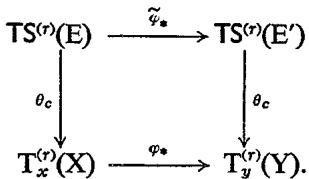
\includegraphics[keepaspectratio]{images/part001_e22e7577.jpg}}

该映射与 \(c\) 和 \(c'\) 的选取无关。若 \(t \in \mathrm{T}_{x}^{(r)}(\mathbf{X})\)，则称 \(\varphi_{*}(t)\) 为 \(t\) 经 \(\varphi\) 得到的像。我们有 \(\varphi_{*}(\varepsilon_{x}) = \varepsilon_{y}\)。若 \(k \leqslant r\)，则有

\[
\varphi_ {*} (\mathrm{T} _ {x} ^ {(k)} (\mathrm{X})) \subset \mathrm{T} _ {y} ^ {(k)} (\mathrm{Y}) \quad \text { and } \quad \varphi_ {*} (\mathrm{T} _ {x} ^ {(k) +} (\mathrm{X})) \subset \mathrm{T} _ {y} ^ {(k) +} (\mathrm{Y}).
\]

若 \(\varphi': X \to Y\) 是一个 \(C^r\) 类态射，且满足 \(\varphi'(x)=y\)，则 \(\varphi_* = \varphi_*'\) 当且仅当 \(j_x^r(\varphi) = j_x^r(\varphi')\)（参见 12.1）。

若 \(\varphi\) 在 \(x, \varphi_*\) 处是一个浸入（相应地，一个浸没），则它是单射（相应地，满射）；当 \(\dim_y Y < +\infty\) 时逆命题成立。

若 \(\varphi'\colon\mathbf{Y}\to\mathbf{Z}\) 是一个 \(\mathbf{C}^{r}\) 类流形态射，且 \(t\in\mathbf{T}_{x}^{(r)}(\mathbf{X})\)，则有 \((\varphi'\circ\varphi)_{*}(t)=\varphi_{*}^{\prime}(\varphi_{*}(t))\)。

设 F 是一个分离的多范数空间，f 是定义在 y 的一个邻域上、取值于 F 的 \(C^{r}\) 类函数。此时我们有

\[
\langle f, \varphi_ {*} (t) \rangle = \langle f \circ \varphi , t \rangle \quad \text {   for   all   } \quad t \in \mathrm{T} _ {x} ^ {(r)} (\mathrm{X}).\tag{1}
\]

对给定的 \(t\)，关系式 (1)（其中 \(f\) 与 \(F\) 为变量）刻画了 \(\varphi_{*}(t)\)；当 \(\dim_y Y < +\infty\) 时，可以只限于 \(F = K\) 的情形。

13.2.4. 假设 X 是 Banach 空间 E 的一个开子流形。用 \(\varphi_x\) 表示从 X 到 E 的映射 \(y \mapsto y - x\)；卡 \(c = (X, \varphi_x, E)\) 以 \(x\) 为中心。于是 \(\mathrm{T}_x^{(r)}(\mathbf{X})\) 与 \(\mathrm{TS}^{(r)}(\mathbf{E})\) 通过 \(\theta_c^{-1}\) 恒同。特别地，我们有 \(\mathrm{T}_x^{(\infty)}(\mathbf{X}) = \mathrm{TS}(\mathbf{E})\)。

设 F 是一个 Banach 空间，\(u: E \to F\) 是一个连续线性映射，且 \(x \in E\)，\(y \in F\) 满足 \(u(x) = y\)。如上所述，把 \(\mathrm{T}_{x}^{(\infty)}(E)\) 与 TS(E) 恒同，把 \(\mathrm{T}_{y}^{(\infty)}(F)\) 与 TS(F) 恒同。映射

\[
u _ {*} \colon \mathrm{TS(E)} \rightarrow \mathrm{TS(F)} \quad (\text { cf. } 13.2.3)
\]

与由 u 到张量代数的典范扩张所诱导的映射 TS(u) 一致。

13.2.5. 若 \(k \leqslant r\)，用 \(\mathrm{T}^{(k)}(\mathrm{X})\)（相应地，\(\mathrm{T}^{(k)+}(\mathrm{X})\)）表示诸 \(\mathrm{T}_a^{(k)}(\mathrm{X})\)（相应地，诸 \(\mathrm{T}_a^{(k)+}(\mathrm{X})\)，其中 \(a \in \mathrm{X}\)）的集合和。映射 \(t: \mathrm{X} \to \mathrm{T}^{(k)}(\mathrm{X})\) 若满足 \(t(a) \in \mathrm{T}_a^{(k)}(\mathrm{X})\)（对一切 \(a \in \mathrm{X}\)），则称为阶 \(\leqslant k\) 的点分布场。

假设 \(k\) 有限且 X 局部有限维。对每个 \(a \in X\)，双线性形式 \((j, t) \mapsto \langle j, t \rangle\)（参见 13.2.2）定义了一个同构 \(i_a\)，它把 \(\mathrm{T}_a^{(k)}(\mathrm{X})\) 映到 \(\mathrm{P}_a^k(\mathrm{X})^*\) 即 \(\mathrm{P}_a^k(\mathrm{X})\) 的对偶上。这些 \(i_a\) 定义了一个双射 \(i: \mathrm{T}^{(k)}(\mathrm{X}) \to \mathrm{P}^k(\mathrm{X})^*\)，其中 \(\mathrm{P}^k(\mathrm{X})^*\) 表示向量丛 \(\mathrm{P}^k(\mathrm{X})\) 的对偶；经由 \(i^{-1}\) 转移结构，我们给 \(\mathrm{T}^{(k)}(\mathrm{X})\) 装备一个以 X 为底、类为 \(\mathbf{C}^{r-k}\) 的向量丛结构。阶 \(\leqslant k\) 的点分布场称为 \(\mathbf{C}^s\) 类的（其中 \(s \leqslant r - k\)），如果它是 \(\mathbf{C}^s\) 类截面，即丛 \(\mathrm{T}^{(k)}(\mathrm{X})\) 的截面。

设 \(\varphi\colon\mathbf{X}\to\mathbf{Y}\) 是一个 \(\mathbf{C}^{r}\) 类流形态射，并假设 Y 与 X 一样是局部有限维的。那么 \(\varphi_{*}\colon\mathrm{T}^{(k)}(\mathrm{X})\to\mathrm{T}^{(k)}(\mathrm{Y})\) 是一个向量丛的 \(\varphi\)-态射，其类为 \(\mathbf{C}^{r-k}\)。

13.2.6. 设 \(k\) 是满足 \(0 \leqslant k \leqslant r\) 的整数。若 U 是有限维 Banach 空间 E 的一个开集，则依据 13.2.4，向量丛 \(\mathbf{T}^{(k)}(\mathbf{U})\) 与以 \(\mathbf{TS}^{(k)}(\mathbf{E})\) 为纤维的平凡丛恒同。

特别地，取 \(E = K^n\)，其中 \(n \geqslant 0\)，并设 \((e_1, \ldots, e_n)\) 为 \(E\) 的典范基。若 \(\alpha = (\alpha_1, \ldots, \alpha_n)\) 是 \(N^n\) 的一个元素，用 \(\Delta^\alpha\) 表示元素 \(\gamma_{\alpha_1}(e_1) \ldots \gamma_{\alpha_n}(e_n)\)（\(TS(E)\) 中的元素，所用的乘积是对称张量的对称积，参见 A, IV, § 5, no. 3）。\(^{(1)}\) 诸 \(\Delta^\alpha\)（其中 \(|\alpha| \leqslant k\)）构成 \(TS^{(k)}(E)\) 的一个基；若 \(a \in K^n\)，用 \(\Delta_a^\alpha\) 表示 \(T_a^{(k)}(E)\) 中相应的元素。设 F 是一个分离的多范数空间，f 是 \(C^r\) 类、定义在 \(a\) 的一个邻域内且取值于 F 的函数；若 \(\alpha \in N^n\)，则元素 \(\langle f, \Delta_a^\alpha \rangle\) 与 2.5.3、3.2.1 和 4.2.1 中定义的元素 \((\Delta^\alpha f)(a)\) 一致。

假设 X 局部有限维，并设 \(\xi = (\xi^1, \ldots, \xi^n)\) 是 X 在开集 U 上的一个坐标系。若 \(a \in \mathbf{U}\) 且 \(\alpha\) 是满足 \(|\alpha| \leqslant k\) 的多重指标，则用 \((\Delta_{\xi}^{\alpha})_a\) 表示点 \(a\) 处这样的点分布：它在 \(\xi\) 下的像是点分布 \(\Delta_{\xi(a)}^{\alpha}\)（在 \(\mathbf{K}^n\) 上）；分布场

\[
\Delta_ {\xi} ^ {\alpha}: a \mapsto (\Delta_ {\xi} ^ {\alpha}) _ {a} \quad (| \alpha | \leqslant k)
\]

构成向量丛 \(\mathbf{T}^{(k)}(\mathbf{X})\) 在 U 上的一个标架。若 \(f\colon \mathbf{U}\to \mathbf{F}\) 是 \(\mathbf{C}^r\) 类的，我们令 \(\langle f, (\Delta_{\xi}^{\alpha})_a\rangle = \Delta_{\xi}^{\alpha}f(a)\)，并用 \(\Delta_{\xi}^{\alpha}f\) 表示函数 \(a\mapsto \Delta_{\xi}^{\alpha}f(a)\)；它是 U 上的一个 \(\mathbf{C}^{r - k}\) 类函数。

\(^{1}\) 若 \(m = |\alpha|\)，且 \(\Sigma\) 是映射 \(\sigma\)（从 \(\{1, \ldots, m\}\) 到 \(\{1, \ldots, n\}\)、满足 \(\operatorname{Card}\sigma^{-1}(i)=\alpha_i\)）全体的集合，则有

\[
\Delta^ {\alpha} = \gamma_{\alpha_1}(e_1) \dots \gamma_{\alpha_n}(e_n) = \sum_{\sigma \in \Sigma} e_{\sigma(1)} \otimes \dots \otimes e_{\sigma(n)}, \quad \text { cf. A, IV, } \S 5, \text { no. } 4.
\]

\subsection{点分布与切空间}

在本节中，X 表示一个 C \(^{r}\) 类流形。

13.3.1. 设 \(x \in X\)，并设 \(k\) 是一个 \(\leqslant r\) 的整数。设 \(c = (U, \varphi, E)\) 是 \(X\) 的以 \(x\) 为中心的一个卡；13.2.1 中定义的同构 \(\theta_c \colon \mathsf{TS}^{(r)}(E) \to \mathsf{T}_x^{(r)}(X)\) 把 \(\mathsf{TS}^{(k)}(E)\) 映到 \(\mathsf{T}_x^{(k)}(X)\) 上，把 \(\mathsf{TS}^{(k-1)}(E)\) 映到 \(\mathsf{T}_x^{(k-1)}(X)\) 上；通过取限制和取商，它诱导出同构

\[
\theta_ {c, k} \colon \mathsf {T S} ^ {k} (\mathrm{E}) = \mathsf {T S} ^ {(k)} (\mathrm{E}) / \mathsf {T S} ^ {(k - 1)} (\mathrm{E}) \rightarrow \mathsf {T} _ {x} ^ {(k)} (\mathrm{X}) / \mathsf {T} _ {x} ^ {(k - 1)} (\mathrm{X}).
\]

另一方面，c 定义了一个同构，仍记作 \(\theta_{c}\)（参见 5.5.1），它把 E 映到切空间 \(T_{x}(X)\) 上。用 \(i_{k}\) 表示复合映射

\[
\mathrm{T} _ {x} ^ {(k)} (\mathrm{X}) / \mathrm{T} _ {x} ^ {(k - 1)} (\mathrm{X}) \xrightarrow {\theta_ {c , k} ^ {- 1}} \mathrm{TS} ^ {k} (\mathrm{E}) \xrightarrow {\mathrm{TS} ^ {k} (\theta_ {c})} \mathrm{TS} ^ {k} (\mathrm{T} _ {x} (\mathrm{X})).
\]

同构 \(i_k\) 与 \(c\) 的选取无关；当 \(k = 1\) 时，用它把 \(\mathrm{T}_x^{(1)+}(\mathrm{X}) = \mathrm{T}_x^{(1)}(\mathrm{X}) / \mathrm{T}_x^{(0)}(\mathrm{X})\) 与切空间 \(\mathrm{T}_x(\mathrm{X})\) 恒同。若 \(t \in \mathrm{T}_x^{(k)}(\mathrm{X})\)，可以把 \(i_k(t)\) 记为 \(i_k\) 作用于 \(t\) 模 \(\mathrm{T}_x^{(k-1)}(\mathrm{X})\) 的类而得的像。

令

\[
\operatorname{gr} _ {k} \mathrm{T} _ {x} ^ {(r)} (\mathrm{X}) = \mathrm{T} _ {x} ^ {(k)} (\mathrm{X}) / \mathrm{T} _ {x} ^ {(k - 1)} (\mathrm{X}) \quad \text { and } \quad \operatorname{gr} \mathrm{T} _ {x} ^ {(r)} (\mathrm{X}) = \bigoplus_ {0 \leqslant k \leqslant r} \operatorname{gr} _ {k} \mathrm{T} ^ {(r)} (\mathrm{X}).
\]

我们称 gr \(\mathbf{T}_{x}^{(r)}(\mathbf{X})\) 为与滤链 \((\mathbf{T}_{x}^{(k)}(\mathbf{X}))_{k\leq r}\)（\(\mathbf{T}_{x}^{(r)}(\mathbf{X})\) 的递增滤链）相伴的分次对象。诸 \(i_k\) 定义了一个分次向量空间的同构

\[
i \colon \operatorname{gr} \mathrm{T} _ {x} ^ {(r)} (\mathrm{X}) \rightarrow \mathrm{TS} ^ {(r)} (\mathrm{T} _ {x} (\mathrm{X})).
\]

若 \(r = \infty\) 或 \(\omega\)，则 \(i\) 是 gr \(T_x^{(r)}(X)\) 到 \(TS(T_x(X))\) 上的同构。当希望指明 \(x\)（或 X，或两者）时，就写 \(i_x\)（或 \(i_X\)，或 \(i_{X,x}\)）以代替 \(i\)。

13.3.2. 在上述假设之外，再假设 X 局部有限维。相对于 X 各点的诸同构 \(i_{k}\) 定义了一个向量丛同构

\[
i _ {k} \colon \mathrm{T} ^ {(k)} (\mathrm{X}) / \mathrm{T} ^ {(k - 1)} (\mathrm{X}) \rightarrow \mathrm{TS} ^ {k} (\mathrm{T} (\mathrm{X}))
\]

其中 TS \(^{k}\) (T(X)) 表示 C \(^{r-1}\) 类的、由有限维向量函子 TS \(^{k}\) 从 T(X) 得到的向量丛（参见 7.6.5）。当 \(k \geqslant 1\) 时，\(i_{k}\) 是一个 C \(^{r-k}\) 类同构；当 \(k = 0\) 时，它是平凡丛 \(\mathrm{K}_{\mathrm{X}}\) 的恒同映射。

13.3.3. 例。—— 在上述假设下，设 \(\xi = (\xi^{1}, \ldots, \xi^{n})\) 是 X 在 \(x\) 处的一个坐标系。用 \((\partial_{i,x})_{1 \leqslant i \leqslant n}\) 表示 \(\mathrm{T}_{x}(\mathrm{X})\) 的由 \(\xi\) 定义的基（参见 5.5.8），并用 \(((\Delta_{\xi}^{\infty})_{x})_{|\alpha| \leqslant k}\) 表示 13.2.6 中定义的 \(\mathrm{T}_{x}^{(k)}(\mathrm{X})\) 的基。我们有：

\[
\begin{array}{l l} i _ {k} ((\Delta_ {\xi} ^ {\alpha}) _ {x}) = 0 & \text {if} \quad | \alpha | <   k \\ i _ {k} ((\Delta_ {\xi} ^ {\alpha}) _ {x}) = \gamma_ {\alpha_ {1}} (\partial_ {1, x}) \dots \gamma_ {\alpha_ {n}} (\partial_ {n, x}) & \text {if} \quad | \alpha | = k. ^ {(1)} \end{array}
\]

\(^{1}\) 这里同样，诸 \(\gamma_{\alpha_{i}}(\partial_{i,x})\) 的乘积是 \(\mathrm{TS}(\mathrm{T}_{x}(\mathrm{X}))\) 中的对称积。

13.3.4. 假设 K 的特征为零，或者 X 局部有限维。设 k 是满足 \(0 \leqslant k \leqslant r\) 的整数，并设 \(x \in X\)；设 F 是一个 Banach 空间。根据 12.6.8，我们有正合序列

\[
0 \rightarrow \mathrm{P} _ {k} (\mathrm{T} _ {x} (\mathrm{X}); \mathrm{F}) \stackrel {{\iota}} {{\rightarrow}} \mathrm{P} _ {x} ^ {k} (\mathrm{F} _ {\mathrm{X}}) \stackrel {{\sigma}} {{\rightarrow}} \mathrm{P} _ {x} ^ {k - 1} (\mathrm{F} _ {\mathrm{X}}) \rightarrow 0,\tag{i}
\]

其中 \(\sigma = r^{k, k-1}\)。另一方面，根据 13.3.1，我们有正合序列

\[
0 \leftarrow \mathsf {T S} ^ {k} (\mathrm{T} _ {x} (\mathrm{X})) \stackrel {{i}} {{\leftarrow}} \mathrm{T} _ {x} ^ {(k)} (\mathrm{X}) \stackrel {{s}} {{\leftarrow}} \mathrm{T} _ {x} ^ {(k - 1)} (\mathrm{X}) \leftarrow 0,\tag{ii}
\]

其中 s 是 \(\mathrm{T}_{x}^{(k-1)}(\mathrm{X})\) 到 \(\mathrm{T}_{x}^{(k)}(\mathrm{X})\) 的包含映射，且 \(i=i_{k}\)。这些正合序列在 F 中“成对”。更确切地说，把它们写成如下形式：

\begin{enumerate}
\def\labelenumi{(\roman{enumi})}
\tightlist
\item
\end{enumerate}

\[
0 \rightarrow \mathrm{A} \xrightarrow {\iota} \mathrm{B} \xrightarrow {\sigma} \mathrm{C} \rightarrow 0\tag{ii}
\]

\[
0 \leftarrow A ^ {\prime} \stackrel {i} {\leftarrow} B ^ {\prime} \stackrel {s} {\leftarrow} C ^ {\prime} \leftarrow 0.
\]

若 \(a \in \mathbf{A}\) 且 \(a' \in \mathbf{A}'\)，F 中的元素 \(\langle a, a' \rangle\) 由 13.1.2 定义；若 \(b \in \mathbf{B}\) 且 \(b' \in \mathbf{B}'\)（相应地，若 \(c \in \mathbf{C}\) 且 \(c' \in \mathbf{C}'\)），F 中的元素 \(\langle b, b' \rangle\)（相应地，\(\langle c, c' \rangle\)）由 13.2.2 定义；于是有：

\[
\langle \iota a, b ^ {\prime} \rangle = \langle a, i b ^ {\prime} \rangle \quad \text { and } \quad \langle \sigma b, c ^ {\prime} \rangle = \langle b, s c ^ {\prime} \rangle \quad \text { if } \quad a \in \mathbf {A}, \quad b \in \mathbf {B}, \quad b ^ {\prime} \in \mathbf {B} ^ {\prime}, \quad c ^ {\prime} \in \mathbf {C} ^ {\prime}.
\]

13.3.5. 设 Y 是一个 \(C^{r}\) 类流形，\(\varphi: X \to Y\) 是一个 \(C^{r}\) 类态射，并设 \(x \in X\)，\(y \in Y\) 满足 \(y = \varphi(x)\)。13.2.3 中定义的映射 \(\varphi_{*}: T_{x}^{(r)}(X) \to T_{y}^{(r)}(Y)\) 与这些空间的滤链相容；通过转到相伴分次对象，它定义了一个线性映射

\[
\operatorname{gr} \left(\varphi_ {*}\right): \operatorname{gr} \mathrm{T} _ {x} ^ {(r)} (\mathrm{X}) \rightarrow \operatorname{gr} \mathrm{T} _ {y} ^ {(r)} (\mathrm{Y}).
\]

我们也用 \(\mathsf{TS}^{(r)}(\mathsf{T}_x(\varphi))\) 表示从 \(\mathsf{TS}^{(r)}(\mathsf{T}_x(\mathbf{X}))\) 到 \(\mathsf{TS}^{(r)}(\mathsf{T}_y(\mathbf{Y}))\) 的、由典范扩张 \(\mathsf{TS}(\mathsf{T}_x(\varphi))\)（\(\mathsf{T}_x(\varphi)\) 的典范扩张）诱导的映射。图表

\[
\begin{array}{c} \operatorname{gr} T _ {x} ^ {(r)} (X) \xrightarrow {\operatorname{gr} (\varphi_ {*})} \operatorname{gr} T _ {y} ^ {(r)} (Y) \\ \Biggl \downarrow i _ {\mathbf {X}, x} \\ \operatorname{TS} ^ {(r)} (T _ {x} (X)) \xrightarrow {\operatorname{TS} ^ {(r)} (T _ {x} (\varphi))} \operatorname{TS} ^ {(r)} (T _ {y} (Y)) \end{array}
\]

是交换的。

13.3.6. 假设 K 的特征为零。利用 A, IV, § 5, no. 8 中定义的同构 \(\varphi_{\mathbb{M}}: \mathsf{S}^k(\mathbf{M}) \to \mathsf{TS}^k(\mathbf{M})\)，可以在前述所有内容中把 \(\mathsf{TS}^k(\mathbf{T}_x(\mathbf{X}))\) 换成 \(k\) 次对称幂 \(\mathsf{S}^k(\mathbf{T}_x(\mathbf{X}))\)，即切空间 \(\mathbf{T}_x(\mathbf{X})\) 的对称幂。

\subsection{点分布的张量积}

13.4.1. 设 \(\mathbf{X}_1\) 与 \(\mathbf{X}_2\) 是两个 \(\mathbf{C}^r\) 类流形，设 \(x_1 \in \mathbf{X}_1\)，\(x_2 \in \mathbf{X}_2\)，以及 \(t_1 \in \mathrm{T}_{x_1}^{(k_1)}(\mathbf{X}_1)\)，\(t_2 \in \mathrm{T}_{x_2}^{(k_2)}(\mathbf{X}_2)\)，其中 \(k_1 + k_2 \leqslant r\)。令 \(\mathbf{X} = \mathbf{X}_1 \times \mathbf{X}_2\)，\(x = (x_1, x_2)\)，\(k = k_{1} + k_{2}\)。对 \(i = 1, 2\)，设 \(c_{i} = (U_{i}, \varphi_{i}, E_{i})\) 是 \(X_{i}\) 的以 \(x_{i}\) 为中心的卡，并用 \(\tilde{t}_{i}\) 表示 \(TS(E_{i})\) 中满足 \(\theta_{c_i}(\tilde{t}_{i}) = t_{i}\) 的元素（参见 13.2.1）。设 \(\sigma\) 是 \(TS(E_{1}) \otimes TS(E_{2})\) 到 \(TS(E_{1} \times E_{2})\) 上的典范同构（参见 A, IV, § 5, no. 5）。元素 \(\sigma(\tilde{t}_{1} \otimes \tilde{t}_{2})\) 是 \(\tilde{t}_{1}\) 与 \(\tilde{t}_{2}\)（视为 \(TS(E_{1} \times E_{2})\) 中的元素，借助典范单射 \(TS(E_{i}) \to TS(E_{1} \times E_{2})\)）的对称积；它属于 \(TS^{(k)}(E_{1} \times E_{2})\)。令 \(c = c_{1} \times c_{2}\)；它是 X 的以 \(x\) 为中心的卡。\(\theta_{c}\) 把 \(\sigma(\tilde{t}_{1} \otimes \tilde{t}_{2})\) 映为 \(T_{x}^{(k)}(X)\) 的一个元素，它与卡 \(c_{i}\) 的选取无关。把它称为 \(t_{1}\) 与 \(t_{2}\) 的直积或对称张量积（甚至简称张量积），并记作 \(t_{1} \times t_{2}\) 或 \(t_{1} \otimes t_{2}\)。

我们有 \(\varepsilon_{x_1} \otimes \varepsilon_{x_2} = \varepsilon_x\)。\(t_1 \otimes t_2\) 的常数项是 \(t_1\) 与 \(t_2\) 的常数项之积。

同构 \((y_{1}, y_{2}) \mapsto (y_{2}, y_{1})\)（从 \(\mathbf{X}_{1} \times \mathbf{X}_{2}\) 到 \(\mathbf{X}_{2} \times \mathbf{X}_{1}\) 上的同构）把 \(t_{1} \otimes t_{2}\) 变为 \(t_{2} \otimes t_{1}\)。

13.4.2（“结合性与函子性”）。设 \(X_{i}\)（i = 1, 2, 3）是 \(C^{r}\) 类流形，并设 \(x_{i} \in X_{i}\)，\(t_{i} \in \mathbf{T}_{x_{i}}^{(k_{i})}(\mathbf{X}_{i})\)，其中 \(k_{1} + k_{2} + k_{3} \leqslant r\)。我们有

\[
\left(t _ {1} \otimes t _ {2}\right) \otimes t _ {3} = t _ {1} \otimes \left(t _ {2} \otimes t _ {3}\right);
\]

把这个点分布记作 \(t_{1} \otimes t_{2} \otimes t_{3}\)。以同样方式定义任意有限的张量积。

设 \(\varphi_{1}\colon\mathbf{X}_{1}\to\mathbf{Y}_{1}\) 与 \(\varphi_{2}\colon\mathbf{X}_{2}\to\mathbf{Y}_{2}\) 是 \(\mathbf{C}^{r}\) 类流形态射，并设 \(t_{1}\in\mathbf{T}^{(k_{1})}(\mathbf{X}_{1})\)，\(t_{2}\in\mathbf{T}^{(k_{2})}(\mathbf{X}_{2})\)，其中 \(k_{1}+k_{2}\leqslant r\)。我们有

\[
(\varphi_ {1} \times \varphi_ {2}) _ {*} (t _ {1} \otimes t _ {2}) = \varphi_ {1 *} (t _ {1}) \otimes \varphi_ {2 *} (t _ {2}).
\]

13.4.3. 沿用 13.4.1 的记号，设 \(F_{1}\)、\(F_{2}\) 与 F 是分离的多范数空间，并设 \((u_{1}, u_{2}) \mapsto u_{1}.u_{2}\) 是从 \(F_{1} \times F_{2}\) 到 F 的一个连续双线性映射。设

\[
f _ {i} \colon \mathrm{X} _ {i} \rightarrow \mathrm{F} _ {i} \quad (i = 1, 2)
\]

是 \(\mathbf{C}^r\) 类映射，并用下式定义 \(f_1 \otimes f_2: \mathbf{X} \to \mathbf{F}\)：

\[
(f _ {1} \otimes f _ {2}) (y _ {1}, y _ {2}) = f _ {1} (y _ {1}). f _ {2} (y _ {2}).
\]

映射 \(f_{1} \otimes f_{2}\) 是 \(\mathbf{C}^{r}\) 类的，且我们有

\[
\langle f _ {1} \otimes f _ {2}, t _ {1} \otimes t _ {2} \rangle = \langle f _ {1}, t _ {1} \rangle . \langle f _ {2}, t _ {2} \rangle .
\]

13.4.4. 沿用 13.4.1 中的记号，设 \(f\) 是从 X 到分离的多范数空间 F 的一个 \(\mathbf{C}^{r}\) 类映射。若 \(y_{1} \in \mathbf{X}_{1}\)，用 \(f_{y_{1}}\) 表示映射 \(y_{2} \mapsto f(y_{1}, y_{2})\)（从 \(\mathbf{X}_{2}\) 到 F 的映射），并令 \(g(y_{1}) = \langle f_{y_{1}}, t_{2} \rangle\)。这样定义的函数 \(g: \mathbf{X}_{1} \to \mathbf{F}\) 是 \(\mathbf{C}^{r - k_{1}}\) 类的，且我们有

\[
\langle f, t _ {1} \otimes t _ {2} \rangle = \langle g, t _ {1} \rangle ,
\]

换言之

\[
\langle f, t _ {1} \otimes t _ {2} \rangle = \langle y _ {1} \mapsto \langle y _ {2} \mapsto f (y _ {1}, y _ {2}), t _ {2} \rangle , t _ {1} \rangle .
\]

同样我们有

\[
\langle f, t _ {1} \otimes t _ {2} \rangle = \langle y _ {2} \mapsto \langle y _ {1} \mapsto f (y _ {1}, y _ {2}), t _ {1} \rangle , t _ {2} \rangle .
\]

13.4.5. 沿用 13.4.1 中的记号，设

\[
\alpha_ {k _ {1}, k _ {2}} \colon \mathrm{T} _ {x _ {1}} ^ {(k _ {1})} (\mathrm{X} _ {1}) \otimes \mathrm{T} _ {x _ {2}} ^ {(k _ {2})} (\mathrm{X} _ {2}) \rightarrow \mathrm{T} _ {x} ^ {(k)} (\mathrm{X})
\]

为由双线性映射 \((t_{1}, t_{2}) \mapsto t_{1} \otimes t_{2}\) 定义的线性映射；该映射是单射；当 \(k_{1}\) 与 \(k_{2}\) 都是无穷时，它是双射。

若 \(n \leqslant r\)，用 \(\mathrm{T}_{x}^{(n)}(\mathrm{X}_{1}, \mathrm{X}_{2})\) 表示 \(\mathrm{T}_{x_{1}}^{(n)}(\mathrm{X}_{1}) \otimes \mathrm{T}_{x_{2}}^{(n)}(\mathrm{X}_{2})\) 中由诸子空间 \(\mathrm{T}_{x_{1}}^{(k_{1})}(\mathrm{X}_{1}) \otimes \mathrm{T}_{x_{2}}^{(k_{2})}(\mathrm{X}_{2})\)（\(k_{1} + k_{2} \leqslant n\)）生成的向量子空间。存在一个线性映射

\[
\alpha_ {n} \colon \mathrm{T} _ {x} ^ {(n)} (\mathrm{X} _ {1}, \mathrm{X} _ {2}) \rightarrow \mathrm{T} _ {x} ^ {(n)} (\mathrm{X})
\]

且是唯一的、延拓上述映射 \(\alpha_{k_1,k_2}\) 的线性映射；它是一个同构。在下文中，我们把 \(\mathrm{T}_x^{(n)}(\mathrm{X})\) 借助 \(\alpha_n^{-1}\) 与 \(\mathrm{T}_x^{(n)}(\mathrm{X}_1,\mathrm{X}_2)\)（\(\mathrm{T}_{x_1}^{(n)}(\mathrm{X}_1)\otimes \mathrm{T}_{x_2}^{(n)}(\mathrm{X}_2)\) 的向量子空间）恒同。

13.4.6. 我们保留 13.4.5 和 13.3.1 的记号。通过取商，\(\alpha_{k_1,k_2}\) 定义了一个线性映射

\[
\varepsilon_ {k _ {1}, k _ {2}} \colon \operatorname{gr} _ {k _ {1}} \mathrm{T} _ {x _ {1}} ^ {(r)} (\mathrm{X} _ {1}) \otimes \operatorname{gr} _ {k _ {2}} \mathrm{T} _ {x _ {2}} ^ {(r)} (\mathrm{X} _ {2}) \rightarrow \operatorname{gr} _ {k} \mathrm{T} _ {x} ^ {(r)} (\mathrm{X}).
\]

诸映射 \(\varepsilon_{k_1,k_2}\)（\(k_1 + k_2 \leqslant r\)）是一个零次分次线性映射的分量

\[
\varepsilon : \bigoplus_ {k _ {1} + k _ {2} \leqslant r} \left(\operatorname{gr} _ {k _ {1}} \mathrm{T} _ {x _ {1}} ^ {(r)} (\mathrm{X} _ {1}) \otimes \operatorname{gr} _ {k _ {2}} \mathrm{T} _ {x _ {2}} ^ {(r)} (\mathrm{X} _ {2})\right)\rightarrow \bigoplus_ {k \leqslant r} \operatorname{gr} _ {k} \mathrm{T} _ {x} ^ {(r)} (\mathrm{X})
\]

且该映射是一个同构。图表

\[
\begin{array}{l} \bigoplus_ {k _ {1} + k _ {2} \leqslant r} (\operatorname{gr} _ {k _ {1}} \mathrm{T} _ {x _ {1}} ^ {(r)} (\mathrm{X} _ {1}) \otimes \operatorname{gr} _ {k _ {2}} \mathrm{T} _ {x _ {2}} ^ {(r)} (\mathrm{X} _ {2})) \xrightarrow {\varepsilon} \operatorname{gr} \mathrm{T} _ {x} ^ {(r)} (\mathrm{X}) \\ \Biggl \downarrow i _ {1 2} \\ \bigoplus_ {k _ {1} + k _ {2} \leqslant r} (\mathrm{TS} ^ {k _ {1}} (\mathrm{T} _ {x _ {1}} (\mathrm{X} _ {1})) \otimes \mathrm{TS} ^ {k _ {2}} (\mathrm{T} _ {x _ {2}} (\mathrm{X} _ {2}))) \xrightarrow {\sigma} \bigoplus_ {k \leqslant r} \mathrm{TS} ^ {k} (\mathrm{T} _ {x _ {1}} (\mathrm{X} _ {1}) \times \mathrm{T} _ {x _ {2}} (\mathrm{X} _ {2})) \end{array}
\]

是交换的（在这个图中，\(i_{12}\) 表示由 \(i_{\mathbf{x}_1} \otimes i_{\mathbf{x}_2}\) 诱导的同态，而 \(\sigma\) 是 A, IV, § 5, no. 5 中定义的同构）。若 \(r\) 是无穷，这个图可以简单地写成：

\[
\begin{array}{l} \operatorname{gr} \mathrm{T} _ {x _ {1}} ^ {(\infty)} (\mathrm{X} _ {1}) \otimes \operatorname{gr} \mathrm{T} _ {x _ {2}} ^ {(\infty)} (\mathrm{X} _ {2}) \xrightarrow {\varepsilon} \operatorname{gr} \mathrm{T} _ {x} ^ {(\infty)} (\mathrm{X}) \\ \Biggl \downarrow_ {i _ {\mathbf {X} _ {1}} \otimes i _ {\mathbf {X} _ {2}}} \\ \operatorname{TS} (\mathrm{T} _ {x _ {1}} (\mathrm{X} _ {1})) \otimes \operatorname{TS} (\mathrm{T} _ {x _ {2}} (\mathrm{X} _ {2})) \xrightarrow {\sigma} \operatorname{TS} (\mathrm{T} _ {x} (\mathrm{X})). \end{array}
\]

\subsection{余积}

在本节中，X 表示一个 \(C^{r}\) 类流形，x 是 X 的一个点。

13.5.1. 设 \(k \leqslant r\)。若 \(\Delta\) 是对角映射 \(y \mapsto (y, y)\)，即从 X 到 \(X \times X\) 的对角映射，则 \(\Delta_*\) 把 \(\mathrm{T}_x^{(k)}(\mathrm{X})\) 映入 \(\mathrm{T}_{(x,x)}^{(k)}(\mathrm{X} \times \mathrm{X})\)，后者是 \(\mathrm{T}_{x}^{(k)}(\mathrm{X})\otimes\mathrm{T}_{x}^{(k)}(\mathrm{X})\) 的一个向量子空间（参见 13.4.5）。这样我们就得到一个线性映射，仍记作 \(\Delta_{*}\)（或 \(c\)）：

\[
\mathrm{T} _ {x} ^ {(k)} (\mathrm{X}) \rightarrow \mathrm{T} _ {x} ^ {(k)} (\mathrm{X}) \otimes \mathrm{T} _ {x} ^ {(k)} (\mathrm{X});
\]

我们把它称为附加于 \(\mathbf{T}_{x}^{(k)}(\mathbf{X})\) 的余积。装备了这个余积之后，\(\mathbf{T}_{x}^{(k)}(\mathbf{X})\) 是一个余结合且余交换的余代数（A, III, p. 144–145）；它以把每个点分布映为其常数项的线性形式（13.2.1）作为余单位。若 \(k' \leqslant k\)，则 \(\mathbf{T}_{x}^{(k')}(\mathbf{X})\) 到 \(\mathbf{T}_{x}^{(k)}(\mathbf{X})\) 的包含映射是余代数的态射。

若 \(c = (\mathrm{U},\varphi ,\mathrm{E})\) 是 \(\mathbf{X}\) 的以 \(x\) 为中心的卡，则同构

\[
\theta_ {c} \colon \mathrm{T} ^ {(k)} (\mathrm{E}) \rightarrow \mathrm{T} _ {x} ^ {(k)} (\mathrm{X})
\]

是一个余代数同构，其中 \(\mathrm{T}^{(k)}(\mathrm{E})\) 装备的是由 TS(E) 的余积诱导的余积（参见 A, IV, § 5, no. 7）。

若 \(\varphi: X \to Y\) 是一个 \(C^r\) 类流形态射，则从 \(T_x^{(k)}(X)\) 到 \(T_{\varphi(x)}^{(k)}(Y)\) 的、由 \(\varphi_*\) 诱导的映射是余代数的态射。

13.5.2. 设 \(F_{1}\)、\(F_{2}\) 与 F 是分离的多范数空间，并设 \((u_{1}, u_{2}) \mapsto u_{1}.u_{2}\) 是从 \(F_{1} \times F_{2}\) 到 F 的一个连续双线性映射。设 \(t \in \mathrm{T}_{x}^{(r)}(\mathrm{X})\)，并设它在余积下的像为 \(\boldsymbol{c}(t) = \sum_{j} u_{j} \otimes v_{j}\)，其中 \(u_{j},v_{j} \in \mathrm{T}_{x}^{(r)}(\mathrm{X})\)。设 \(f_{i}: X \to F_{i}\)（\(i=1,2\)）是 \(C^{r}\) 类映射。我们有

\[
\langle f _ {1}. f _ {2}, t \rangle = \sum_ {j} \langle f _ {1}, u _ {j} \rangle . \langle f _ {2}, v _ {j} \rangle ,
\]

按记号的滥用，我们把它写成：

\[
\langle f _ {1}. f _ {2}, t \rangle = \langle f _ {1} \otimes f _ {2}, c (t) \rangle .
\]

13.5.3. 设 \(t \in \mathbf{T}_x^{(k)}(\mathbf{X})\)，其中 \(k \leqslant r\)。

\begin{enumerate}
\def\labelenumi{\alph{enumi})}
\item
  要使 \(c(t)=t\otimes t\)，必须且只需 \(t\) 等于 0 或等于 \(\varepsilon_{x}\)。
\item
  要使 \(c(t)=t\otimes\varepsilon_{x}+\varepsilon_{x}\otimes t\)，必须且只需 \(t\) 是一个切向量，即 \(t\in\mathrm{T}_{x}^{(1)+}(X)\)。
\end{enumerate}

\subsection{有限支集分布}

13.6.1. 设 X 是一个 \(\mathbf{C}^r\) 类流形，并设 \(k \leqslant r\)。用 \(\mathcal{T}^{(k)}(\mathbf{X})\) 表示诸空间 \(\mathrm{T}_x^{(k)}(\mathbf{X})\)（\(x \in \mathbf{X}\)）的直和。\(\mathcal{T}^{(k)}(\mathbf{X})\) 的元素称为 \(\mathbf{X}\) 上阶 \(\leqslant k\) 的有限支集分布。若 \(f: \mathbf{X} \to \mathbf{F}\) 是 \(\mathbf{C}^r\) 类、取值于分离的多范数空间 \(\mathbf{F}\) 的函数，且 \(t = \sum_{x \in \mathbf{X}} t_x\)（其中 \(t_x \in \mathrm{T}_x^{(k)}(\mathbf{X})\) 对一切 \(x \in \mathbf{X}\) 成立）是一个有限支集分布，则我们令

\[
\langle f, t \rangle = \sum_ {x \in X} \langle f, t _ {x} \rangle .
\]

类似地，我们令 \(c(t) = \sum_{x \in X} c(t_x)\)，这给 \(\mathcal{T}^{(k)}(X)\) 装备了一个以 \(t \mapsto \langle 1, t \rangle\) 为余单位的余结合、余交换余代数结构。包含映射 \(\mathcal{T}^{(k')}(X) \to \mathcal{T}^{(k)}(X)\)（其中 \(k' \leqslant k\)）是余代数的态射。

若 \(\varphi: X \to Y\) 是一个 \(C^r\) 类流形态射，则诸映射 \(\mathrm{T}_x^{(k)}(\varphi): \mathrm{T}_x^{(k)}(X) \to \mathrm{T}_{\varphi(x)}^{(k)}(Y)\)（其中 \(x\) 取遍 \(X\)）定义了一个线性映射 \(\varphi_*\)，它把 \(\mathcal{T}^{(k)}(X)\) 映到 \(\mathcal{T}^{(k)}(Y)\)，且是余代数的态射。

若 \(X_{1}\) 与 \(X_{2}\) 是两个 \(C^{r}\) 类流形，则诸映射 \(\alpha_{k}^{-1}\)（参见 13.4.5）定义了一个线性映射

\[
\mathcal {T} ^ {(k)} \left(\mathrm{X} _ {1} \times \mathrm{X} _ {2}\right)\rightarrow \mathcal {T} ^ {(k)} \left(\mathrm{X} _ {1}\right) \otimes \mathcal {T} ^ {(k)} \left(\mathrm{X} _ {2}\right)
\]

它是单射；它是余代数的态射。若 \(k = \infty\) 或 \(\omega\)，它是余代数的同构。

13.6.2. 设 X 是一个 \(C^{r}\) 类流形，V 是一个有限维 K-向量空间。\(\mathcal{T}^{(r)}(\mathrm{X})\otimes\mathrm{V}\) 的元素称为 X 上取值于 V 的有限支集分布。当 K = R、V = C 时，这样的分布也称为 X 上的复有限支集分布。前面各条的定义和结论通过线性性立即推广到取值于 V 的分布。

\subsection{结构弱化}

我们假设 \(\mathbf{K} = \mathbf{R}\)。设 \(r' \in \mathrm{N}_{\mathbb{K}}\) 满足 \(r' \leqslant r\)。设 X 是一个 \(\mathbf{C}^{r}\) 类流形，\(\mathbf{X}'\) 是通过结构弱化（5.13.1）得到的 \(\mathbf{C}^{r'}\) 类流形。设 \(x \in \mathbf{X}\)，并设 \(t \in \mathrm{T}_x^{(k)}(\mathbf{X})\)，其中 \(k \leqslant r'\)。取 X 的一个卡 \(c = (\mathrm{U}, \varphi, \mathrm{E})\)，其中心为 \(x\)，并用 \(\tilde{t}\) 表示 \(\mathrm{TS}^{(k)}(\mathrm{E})\) 中满足 \(\theta_c(\tilde{t}) = t\) 的元素。由于 \(c\) 也是 \(\mathbf{X}'\) 的以 \(x\) 为中心的卡，元素 \(t' = \theta_c(\tilde{t})\)（\(\mathrm{T}_x^{(k)}(\mathrm{X}')\) 中的元素）有定义；它与 \(c\) 的选取无关。映射 \(t \mapsto t'\) 是 \(\mathrm{T}_x^{(k)}(\mathbf{X})\) 到 \(\mathrm{T}_x^{(k)}(\mathbf{X}')\) 上的一个双射，借助它把这两个空间恒同。这样得到的恒同与前面各条中的运算 \(\langle f, t \rangle\)、\(\varphi_*(t)\)、\(t_1 \otimes t_2\)、\(c(t)\)、\ldots{} 相容。

\section{微分算子}

在本段中，X 表示一个局部有限维的 \(C^{r}\) 类流形，其中 \(r \in N_{K}\)；设 E 与 F 是两个以 X 为底的 \(C^{r}\) 类有限秩向量丛。

所考虑的所有流形和向量丛都假设是局部有限维的。

\subsection{微分算子}

14.1.1. 设 \(k\) 是满足 \(0 \leqslant k \leqslant r\) 的整数，并设 \(\mathbf{P}^k(\mathbf{E})\) 是 E 的 \(k\) 阶截面射流丛（12.6.1）。令

\[
\mathbf {D} ^ {k} (\mathbf {E}, \mathbf {F}) = \mathscr {L} (\mathbf {P} ^ {k} (\mathbf {E}); \mathbf {F}).
\]

它是一个以 X 为底、\(C^{r-k}\) 类的向量丛。这个丛在 X 的开集 U 上的截面等同于一个映射

\[
\mathbf {D}: \mathrm{P} ^ {k} (\mathrm{E}) | \mathrm{U} \rightarrow \mathrm{F} | \mathrm{U}
\]

它与到 U 上的投影交换，且在每个纤维上是线性的；这样的截面称为 U 上的 E \(\to\) F 型、阶 \(\leqslant k\) 的微分算子。设 \(h \in N_{K} \cup \{0\}\)，其中 \(0 \leqslant h \leqslant r-k\)。用 \(\mathcal{D}_{\mathrm{U}}^{k,h}(\mathrm{E}, \mathrm{F})\) 表示 U 上的 E \(\to\) F 型、阶 \(\leqslant k\) 且为 \(C^{h}\) 类（作为 \(\mathrm{D}^{k}(\mathrm{E}, \mathrm{F})\) 的截面，或作为 \(\mathrm{P}^{k}(\mathrm{E})|\mathrm{U}\) 到 \(\mathrm{F}|\mathrm{U}\) 的态射，二者是一回事）的微分算子全体组成的集合。若 \(\mathrm{M} = \mathrm{D}^{k}(\mathrm{E}, \mathrm{F})\)，则有 \(\mathcal{D}_{\mathrm{U}}^{k,h}(\mathrm{E}, \mathrm{F}) = \mathcal{S}_{\mathrm{M}}^{h}(\mathrm{U})\)；它是 \(\mathcal{C}^{h}(\mathrm{U})\) 上的模（参见 7.4.1）。

若 \(0 \leqslant k' \leqslant k\)，则态射 \(r^{k, k'}: \mathrm{P}^{k}(\mathrm{E}) \to \mathrm{P}^{k'}(\mathrm{E})\)（参见 12.6.6）定义了从 \(\mathrm{D}^{k'}(\mathrm{E}, \mathrm{F})\) 到 \(\mathrm{D}^{k}(\mathrm{E}, \mathrm{F})\) 的一个单射；从而每个阶 \(\leqslant k'\) 的微分算子都等同于一个阶 \(\leqslant k\) 的微分算子。一个阶 \(\leqslant k\) 但非阶 \(\leqslant k - 1\) 的微分算子有时称为 \(k\) 阶微分算子。若 \(h \in \mathbf{N}_{\mathbb{K}} \cup \{0\}\) 且 \(h \leqslant r - k\)，且 U 是 X 的开子集，则有：

\[
0 \subset \mathcal {D} _ {\mathrm{U}} ^ {0, h} (\mathrm{E}, \mathrm{F}) \subset \mathcal {D} _ {\mathrm{U}} ^ {1, h} (\mathrm{E}, \mathrm{F}) \subset \dots \subset \mathcal {D} _ {\mathrm{U}} ^ {k, h} (\mathrm{E}, \mathrm{F}).
\]

若 \(r=\infty\) 或 \(\omega\)，用 \(\mathcal{D}_{\mathrm{U}}^{\infty,h}(\mathrm{E},\mathrm{F})\) 表示诸 \(\mathcal{D}_{\mathrm{U}}^{k,h}(\mathrm{E},\mathrm{F})\)（\(k\geqslant0\)）的并；这个并的元素称为 U 上的有界阶微分算子（E \(\rightarrow\) F 型、C \(^{h}\) 类），有时也简称 U 上的微分算子。

14.1.2（“零阶算子”）。我们有 \(\mathbf{P}^0 (\mathbf{E}) = \mathbf{E}\)（12.5.1）以及 \(\mathrm{D}^0 (\mathrm{E},\mathrm{F}) = \mathcal{L}(\mathrm{E};\mathrm{F})\)。若 U 是 X 中的开集，且 \(h\in \mathbf{N}_{\mathbb{K}}\cup \{0\}\)、\(h\leqslant r\)，则 \(\mathcal{D}_{\mathbf{U}}^{0,h}(\mathbf{E},\mathbf{F})\) 的元素是 \(\mathbf{C}^h\) 类的、从 E\textbar U 到 F\textbar U 的态射。

14.1.3（“结构弱化”）。假设 K = R，并设 \(r' \in N_{R}\) 满足 \(r' \leqslant r\)。设 X'、E' 与 F' 分别是由 X、E 与 F 通过弱化结构得到的 \(C^{r'}\) 类流形和向量丛。设 k 是满足 \(0 \leqslant k \leqslant r'\) 的整数。那么 \(P^{k}(E')\) 是一个 \(C^{r'-k}\) 类丛，由 \(P^{k}(E)\) 通过弱化结构得到，对 \(D^{k}(E', F')\) 也有类似的结果。特别地，若 U 是 X 中的开集，且 \(0 \leqslant h \leqslant r - k'\)，则有 \(\mathcal{D}_{\mathrm{U}}^{k,h}(E', F') = \mathcal{D}_{\mathrm{U}}^{k,h}(E, F)\)。

14.1.4. 设 D 是 X 上的一个 E \(\to\) F 型、阶 \(\leqslant k\)（其中 \(0 \leqslant k \leqslant r\)）的微分算子。设 U 是 X 的开子集，s 是 E 在 U 上的一个 \(\mathbf{C}^{m}\) 类截面，其中 \(m \in N _{K} \cup \{0\}\) 且 \(k \leqslant m \leqslant r\)。那么 \(j^{k}(s)\) 是一个 \(\mathbf{C}^{m-k}\) 类截面，即 \(P^{k}(E)\) 在 U 上的截面（12.6.1）；它在 D 下的像记作 \(D_{U}(s)\) 或 D(s)。它是 F 在 U 上的一个截面。假设 D 是 \(\mathbf{C}^{h}\) 类的，其中 \(h=m-k\)。那么 \(D_{U}(s)\) 是 \(\mathbf{C}^{h}\) 类的，且诸映射

\[
\mathrm{D} _ {\mathrm{U}} \colon \mathcal {S} _ {\mathrm{E}} ^ {m} (\mathrm{U}) \rightarrow \mathcal {S} _ {\mathrm{F}} ^ {h} (\mathrm{U})
\]

具有下列性质：

\begin{enumerate}
\def\labelenumi{(\arabic{enumi})}
\item
  \(D_{U}\) 是 K-线性的。
\item
  对每个 \(s \in \mathcal{S}_{\mathbb{E}}^{m}(\mathrm{U})\) 及每个 \(\mathrm{V}\)（\(\mathrm{U}\) 的开集），有 \(\mathrm{D}_{\mathrm{V}}(s|\mathrm{V}) = \mathrm{D}_{\mathrm{U}}(s)|\mathrm{V}\)。
\item
  对每个 \(s \in \mathcal{S}_{\mathbb{E}}^{m}(\mathrm{U})\) 及每个 \(x \in \mathrm{U}\)（满足 \(j_{x}^{k}(s) = 0\)），有 \(D_{\mathrm{U}}(s)(x) = 0\)。
\end{enumerate}

(3') 对 U 内每个坐标系 \(\xi = (\xi^1, \ldots, \xi^n)\) 以及 E 在 U 上的任意标架 \(s = (s_1, \ldots, s_d)\)（7.4.4），存在 F 在 U 上的截面 \(n_{i,\alpha}(1 \leqslant i \leqslant d, \alpha \in \mathbf{N}^n, |\alpha| \leqslant k)\)（\(C^h\) 类的截面），使得对每个族 \((f_i)_{1 \leqslant i \leqslant d}\)（\(\mathcal{C}^m(U)\) 中元素的族），有

\[
\mathrm{D} _ {\mathrm{U}} \left(\sum_ {1 \leqslant i \leqslant d} f _ {i}. s _ {i}\right) = \sum_ {1 \leqslant i \leqslant d, | \alpha | \leqslant k} \Delta_ {\xi} ^ {\alpha} (f _ {i}). n _ {i, \alpha},
\]

\begin{enumerate}
\def\labelenumi{(\arabic{enumi})}
\setcounter{enumi}{3}
\tightlist
\item
  对任意函数 \(f \in \mathcal{C}^m(\mathrm{U})\) 及任意映射 \(\theta\)（从 \(\mathcal{S}_{\mathrm{U}}^{m}(\mathrm{E})\) 到 \(\mathcal{S}_{\mathrm{U}}^{h}(\mathrm{F})\)），用 \(\operatorname{ad}(f)\theta\) 表示映射
\end{enumerate}

\[
s \mapsto f. \theta (s) - \theta (f. s)
\]

（从 \(\mathcal{S}_{\mathrm{U}}^{m}(\mathrm{E})\) 到 \(\mathcal{S}_{\mathrm{U}}^{h}(\mathrm{F})\)）。那么，对每个函数 \(f \in \mathcal{C}^{m}(\mathrm{U})\)，存在一个微分算子 \(\mathbf{L}\)（\(\mathbf{U}\) 上的算子），它是 \(\mathrm{E} \to \mathrm{F}\) 型、阶 \(\leqslant k - 1\) 且 \(\mathbf{C}^{h}\) 类的，使得

\[
(\operatorname{ad} (f) \mathrm{D} _ {\mathrm{U}}) (s) = \mathrm{L} _{\mathrm{U}}(s) \quad \text { for all } s \in \mathscr{S}_{\mathrm{E}}^{m}(\mathrm{U}).
\]

\begin{enumerate}
\def\labelenumi{(\arabic{enumi})}
\setcounter{enumi}{4}
\tightlist
\item
  我们有
\end{enumerate}

\[
\operatorname{ad} (f _ {0}) \dots \operatorname{ad} (f _ {k}) \mathrm{D} _ {\mathrm{U}} = 0 \quad \text { for all } f _ {0}, \dots , f _ {k} \text { in } \mathscr {C} ^ {m} (\mathrm{U}).
\]

若令 I = \{0, . . ., k\}，并对 I 的每个子集 H 令 \(f_{H} = \prod_{i \in H} f_i\)，则前面的关系式等价于：

\[
\sum_ {\mathrm{H} \in \mathrm{I}} (- 1) ^ {\operatorname{Card} (\mathrm{H})} f _ {\mathrm{H}}. \mathrm{D} _ {\mathrm{U}} (f _ {\mathrm{I-H}}. s) = 0
\]

其中 \(f_{0},\ldots,f_{k}\) 取遍 \(\mathcal{C}^{m}(\mathrm{U})\)，\(s\) 取遍 \(\mathcal{S}_{\mathbf{E}}^{m}(\mathrm{U})\)。

14.1.5（“微分算子的刻画”）。设 \(k, m\) 与 \(h = m - k\) 如 14.1.4 所述。对 X 的每个开集 U，设 \(\mathbf{D}_{\mathbf{U}}\) 是从 \(\mathcal{S}_{\mathbf{E}}^{m}(\mathbf{U})\) 到 \(\mathcal{S}_{\mathbf{F}}^{h}(\mathbf{U})\) 的一个映射。假设对 X 的每个开子集 U，14.1.4 的条件 1、2、3（相应地，1、2、3'）都满足。那么存在 \(\mathcal{D}_{\mathbf{X}}^{k,h}(\mathbf{E},\mathbf{F})\) 中唯一的元素 D，使得诸 \(\mathbf{D}_{\mathbf{U}}\) 是相应的映射。\(^{(1)}\) 在下文中，我们把 D 与诸 \(\mathbf{D}_{\mathbf{U}}\) 组成的族恒同。

当 \(m = \infty\) 或 \(\omega\) 时，有 \(h = m\)，并且可以把条件 (3) 与 (3') 换成条件 (4) 或 (5) 之一。

14.1.6（“标量算子”）。假设 E 与 F 都等于平凡丛 \(K_{X}\)。这时 \(E \rightarrow F\) 型的微分算子称为标量微分算子，或简称微分算子；若它是阶 \(\leqslant k\) 的，则它是丛 \(\mathcal{L}(\mathrm{P}^{k}(\mathrm{X}); \mathrm{K}_{\mathrm{X}}) = \mathrm{P}^{k}(\mathrm{X})^{*}\)（丛 \(\mathrm{P}^{k}(\mathrm{X})\) 的对偶）的截面；利用同构

\[
i ^ {- 1} \colon \mathrm{P} ^ {k} (\mathrm{X}) ^ {*} \rightarrow \mathrm{T} ^ {(k)} (\mathrm{X}) \quad (\text { cf. } 13.2.5),
\]

可知阶 \(\leqslant k\) 的标量微分算子等同于向量丛 \(\mathbf{T}^{(k)}(\mathbf{X})\) 的截面，即阶 \(\leqslant k\) 的点分布场。

特别地，取 X 为 \(K^{n}\) 的一个开集，其中 n 是一个 \(\geqslant0\) 的整数。点分布场

\[
\Delta^ {\alpha} \colon x \mapsto \Delta_ {x} ^ {\alpha} \quad (\text { cf. } 1 3. 2. 6)
\]

都是 \(\mathbf{C}^{\omega}\) 类的标量微分算子。对每个 \(h\in\mathbf{N}_{\mathbf{K}}\)，诸 \(\Delta^{\alpha}\)（\((|\alpha|\leqslant k)\)）构成 \(\mathcal{C}^{h}(\mathbf{X})\)-模 \(\mathcal{D}_{\mathbf{X}}^{k,h}(\mathbf{K}_{\mathbf{X}},\mathbf{K}_{\mathbf{X}})\) 的一个基。

14.1.7（“实流形上的复微分算子”）。假设 K = R，且向量丛 E 与 F 都装备了复结构（8.8.1）；设 k 是满足 \(0 \leqslant k \leqslant r\) 的整数。这时丛 \(\mathrm{P}^{k}(\mathrm{E})\) 装备有一个复结构（12.6.3）；丛 \(\mathcal{L}_{\mathbf{C}}(\mathrm{P}^{k}(\mathrm{E}); \mathrm{F})\)（7.8.5，由 \(\mathrm{P}^{k}(\mathrm{E})\) 到 F 的复线性映射组成的丛）是 \(\mathcal{L}(\mathrm{P}^{k}(\mathrm{E}); \mathrm{F}) = \mathrm{D}^{k}(\mathrm{E}, \mathrm{F})\) 的一个向量子丛；我们把它记作 \(\mathrm{D}_{\mathbf{C}}^{k}(\mathrm{E}, \mathrm{F})\)。\(\mathrm{D}_{\mathbf{C}}^{k}(\mathrm{E}, \mathrm{F})\) 的截面称为 \(E \to F\) 型、阶 \(\leqslant k\) 的复微分算子。若 \(h \in N_{K}\) 且 \(h \leqslant r - k\)，且 U 是 X 的开集，我们类似地用 \(\mathcal{D}_{\mathbf{U}}^{k,h}(\mathrm{E}, \mathrm{F})_{\mathbf{C}}\) 表示 \(C^{h}\) 类截面（\(\mathrm{D}_{\mathbf{C}}^{k}(\mathrm{E}, \mathrm{F})\) 在 U 上的截面）所成的空间；它是一个 C-向量空间。本段的其他定义和结论类似地推广到复微分算子；其表述留给读者。

14.1.8（“复合”）。设 G 是一个以 X 为底的 \(C^{r}\) 类向量丛。设 \(k'\) 与 \(k''\) 是正整数，其和 \(k \leqslant r\)，并设 \(D'\)（相应地，\(D''\)）是 X 上的一个 \(E \to F\) 型（相应地，\(F \to G\) 型）、阶 \(\leqslant k'\)（相应地，\(\leqslant k''\)）的微分算子。假设 \(D': P^{k'}(E) \to F\) 是 \(C^{h'}\) 类的，其中 \(h' \in N_{K} \cup \{0\}\) 且 \(k'' \leqslant h' \leqslant r - k'\)；映射

\[
\mathbf {D} _ {*} ^ {\prime} = \mathbf {P} ^ {k ^ {\prime \prime}} (\mathbf {D} ^ {\prime}) \colon \mathbf {P} ^ {k ^ {\prime \prime}} (\mathbf {P} ^ {k ^ {\prime}} (\mathbf {E})) \rightarrow \mathbf {P} ^ {k ^ {\prime \prime}} (\mathbf {F})
\]

该映射是 \(\mathbf{C}^{h'-k''}\) 类的（12.6.3）。设 \(\beta\) 是从 \(\mathbf{P}^{k}(\mathbf{E})\) 到 \(\mathbf{P}^{k''}(\mathbf{P}^{k'}(\mathbf{E}))\) 的典范同态（参见 12.6.5）。把映射

\[
\mathrm{P} ^ {k} (\mathrm{E}) \xrightarrow {\beta} \mathrm{P} ^ {k ^ {\prime \prime}} (\mathrm{P} ^ {k ^ {\prime}} (\mathrm{E})) \xrightarrow {\mathrm{D} _ {*} ^ {\prime}} \mathrm{P} ^ {k ^ {\prime \prime}} (\mathrm{F}) \xrightarrow {\mathrm{D} ^ {\prime \prime}} \mathrm{G},
\]

复合起来，就得到一个 E → G 型、阶 ≤ k 的微分算子。这个算子称为 D'' 与 D' 的复合；记作 D'' ∘ D'。

\(^{1}\) 此外，只需条件 (3′) 对一个坐标系族 \((\xi_{\lambda})\) 和一个定义域覆盖 X 的标架族 \((s_{\lambda})\) 满足即可。

若 U 是 X 的开子集，且 \(s \in \mathcal{S}_{\mathrm{E}}^{k}(\mathrm{U})\)，则有

\[
(\mathbf {D} ^ {\prime \prime} \circ \mathbf {D} ^ {\prime}) (s) = \mathbf {D} ^ {\prime \prime} (\mathbf {D} ^ {\prime} (s))
\]

（其中两边都是 G 在 U 上的截面）；这印证了所采用的术语和记号。

现在假设 \(\mathbf{D}^{\prime \prime}\) 是 \(\mathbf{C}^{h^{\prime \prime}}\) 类的，其中 \(h^{\prime \prime} \in \mathrm{N}_{\mathbb{K}} \cup \{0\}\) 且 \(h^{\prime \prime} \leqslant r-k^{\prime\prime}\)。那么 \(\mathbf{D}^{\prime \prime} \circ \mathbf{D}^{\prime}\) 是 \(\mathbf{C}^{h}\) 类的，其中 \(h=\inf(h'-k'',h'')\)。

假设 E = F = G，且 \(k' \leqslant h''\)，此时 \(D' \circ D''\) 有定义。那么 \(D' \circ D'' - D'' \circ D'\) 是一个 \(E \to E\) 型、阶 \(\leqslant k - 1\) 的微分算子；我们把它记作 \([D', D'']\)。

14.1.9（“结合性”）。沿用 14.1.8 的记号与假设，设 H 是一个 \(\mathbf{C}^r\) 类、以 X 为底的向量丛，并设 \(\mathbf{D}''\) 是 X 上的一个 \(\mathbf{G} \to \mathbf{H}\) 型、阶 \(\leqslant k^{m}\) 的微分算子，其中 \(k' + k'' + k'' \leqslant r\)。我们假设 \(\mathbf{D}'\) 是 \(\mathbf{C}^{h'}\) 类的，其中 \(h' \in \mathrm{N}_{\kappa} \cup \{0\}\) 且 \(k'' + k'' \leqslant h' \leqslant r - k'\)；并假设 \(\mathbf{D}''\) 是 \(\mathbf{C}^{h''}\) 类的，其中 \(h'' \in \mathrm{N}_{\kappa} \cup \{0\}\) 且 \(k'' \leqslant h'' \leqslant r - k''\)。那么复合

\[
\mathbf {D} ^ {\prime \prime \prime} \circ (\mathbf {D} ^ {\prime \prime} \circ \mathbf {D} ^ {\prime}) \quad \text { and } \quad (\mathbf {D} ^ {\prime \prime \prime} \circ \mathbf {D} ^ {\prime \prime}) \circ \mathbf {D} ^ {\prime}
\]

都有定义并且相等。

14.1.10. 例子

\begin{enumerate}
\def\labelenumi{\alph{enumi})}
\tightlist
\item
  设 U 是 X 的开子集，\(D \in \mathcal{D}_{\mathrm{U}}^{k,h}(\mathrm{E}, \mathrm{F})\)，其中 \(h \in N_{K} \cup \{0\}\) 且 \(h \leqslant r-k\)，并设 \(f \in \mathcal{C}^{h+k}(\mathrm{U})\)（相应地，\(f \in \mathcal{C}^{h}(\mathrm{U})\)）。E（相应地，F）中乘以 f 的运算是 U 上的一个阶 \(\leqslant0\)、E \(\to\) E 型（相应地，F \(\to\) F 型）的微分算子（参见 14.1.2）。复合 \(D\circ f\) 与 \(f\circ D\) 有定义且属于 \(\mathcal{D}_{\mathrm{U}}^{k,h}(\mathrm{E},\mathrm{F})\)；我们令
\end{enumerate}

\[
\operatorname{ad} (f) \mathrm{D} = f \circ \mathrm{D} - \mathrm{D} \circ f \in \mathcal {D} _ {\mathrm{U}} ^ {k - 1, h} (\mathrm{E}, \mathrm{F}),
\]

（参见 14.1.4, (4)）。这样就给 \(\mathcal{D}_{\mathrm{U}}^{k,h}(\mathrm{E},\mathrm{F})\) 装备了一个右 \(\mathcal{C}^{h+k}(\mathrm{U})\)-模（相应地，左 \(\mathcal{C}^h (\mathrm{U})\)-模）结构。左模结构与 14.1.1 中的一致。

\begin{enumerate}
\def\labelenumi{\alph{enumi})}
\setcounter{enumi}{1}
\item
  假设 \(r = \infty\) 或 \(r = \omega\)。\(E \to E\) 型、\(C^r\) 类的微分算子构成一个含幺元素的结合 K-代数。
\item
  取 X 为 \(K^{n}\) 的一个开子集。标量微分算子 \(\Delta^{\alpha}\)（14.1.6）满足公式
\end{enumerate}

\[
\Delta^ {\alpha} \circ \Delta^ {\beta} = ((\alpha , \beta)) \Delta^ {\alpha + \beta}.
\]

它们彼此交换。用 \(D_{i}\) 表示算子 \(\Delta^{\varepsilon_{i}}\)（“第 i 个偏导数”）。若 K 的特征为 0，我们有

\[
\Delta^ {\alpha} = \frac {1}{\alpha !} D _ {1} ^ {\alpha_{1}} \dots D _ {n} ^ {\alpha_{n}}.
\]

若 K 的特征为 \(p \neq 0\)，则有 \(\mathbf{D}_{i}^{p} = 0\)（对一切 \(i\)）。

14.1.11（“多微分算子”）。设 \(E_{1}, \ldots, E_{n}\) 是以 X 为底的 \(C^{r}\) 类向量丛，并设 \(k, k_{1}, \ldots, k_{n}\) 是属于 \([0, r]\) 的整数。令

\[
\mathrm{L} (k _ {1}, \dots , k _ {n}) = \mathscr {L} (\mathrm{P} ^ {k _ {1}} (\mathrm{E} _ {1}) \otimes \dots \otimes \mathrm{P} ^ {k _ {n}} (\mathrm{E} _ {n}); \mathrm{F}).
\]

若 \(k_i \leqslant k\)（对一切 \(i\)），则投影 \(r^k, k_i: \mathrm{P}^k(\mathrm{E}_i) \to \mathrm{P}^{k_i}(\mathrm{E}_i)\) 使我们能把丛 \(\mathrm{L}(k_1, \ldots, k_n)\) 等同于丛 \(\mathrm{L}(k) = \mathrm{L}(k, \ldots, k)\) 的一个子丛。存在最小子丛 \(\mathrm{M}(k)\)（\(\mathrm{L}(k)\) 的子丛），它包含所有子丛 \(\mathrm{L}(k_1, \ldots, k_n)\)（\(k_1 + \cdots + k_n = k\)）。截面 \(\mathrm{H}\)（\(\mathrm{M}(k)\) 的截面）称为 \((\mathrm{E}_1, \ldots, \mathrm{E}_n) \to \mathrm{F}\) 型、阶 \(\leqslant k\) 的 n-微分算子（或多微分算子）。若 \(s_i\)（\(1 \leqslant i \leqslant n\)）是 \(\mathbf{C}^m (m \in \mathbb{N}_{\mathbb{K}}, m \geqslant k)\) 类截面（\(\mathbf{E}_i\) 在 X 的开集 U 上的截面），则把 \(\mathrm{H}_{\mathrm{U}}(s_1, \ldots, s_n) = \mathrm{H}(s_1, \ldots, s_n)\) 定义为下述丛的截面 \(j^k(s_1) \otimes \cdots \otimes j^k(s_n)\) 在 H 下的像：

\[
\mathbf {P} ^ {k} (\mathrm{E} _ {1}) \otimes \dots \otimes \mathbf {P} ^ {k} (\mathrm{E} _ {n}).
\]

它是 F\textbar U 的一个截面。若 H 是 \(\mathbf{C}^h\) 类的，则该截面是 \(\mathbf{C}^p\) 类的，其中 \(p = \inf(m - k, h)\)。

当 \(E_{1}, \ldots, E_{n}\) 与 F 都等于 \(K_{x}\) 时，称 H 为标量 n-微分算子（或标量多微分算子）。

例。—— 设 J 是一个有限集，X 是 K \(^{J}\) 的一个开子集。设 H 是 X 上的一个阶 \(\leqslant k\) 的标量 n-微分算子。存在唯一的标量函数族

\[
c (\alpha (1), \dots , \alpha (n)) _ {(\alpha (1), \dots , \alpha (n)) \in \mathbf {N} ^ {\mathrm{J}}}, \quad \sum_ {i = 1} ^ {n} | \alpha (i) | \leqslant k
\]

（定义在 X 上），使得

\[
\mathrm{H} _ {\mathrm{X}} \left(f _ {1}, \dots , f _ {n}\right) = \sum_ {\alpha (1), \dots , \alpha (n)} c (\alpha (1), \dots , \alpha (n)) \Delta^ {\alpha (1)} \left(f _ {1}\right) \dots \Delta^ {\alpha (n)} \left(f _ {n}\right)
\]

对每个函数族 \((f_1, \ldots, f_n)\)（\(\mathbf{C}^k\) 类函数族，\(X\) 上的）成立。要使 \(H\) 是 \(\mathbf{C}^h\) 类的，必须且只需诸函数 \(c(\alpha(1), \ldots, \alpha(n))\) 是 \(\mathbf{C}^h\) 类的。

\subsection{符号}

14.2.1. 设 \(k\) 是一个 \(\leqslant r\) 的正整数。考虑正合序列

\[
0 \rightarrow \mathrm{P} _ {k} (\mathrm{T} (\mathrm{X}); \mathrm{E}) \xrightarrow {\iota} \mathrm{P} ^ {k} (\mathrm{E}) \xrightarrow {\jmath} \mathrm{P} ^ {k - 1} (\mathrm{E}) \rightarrow 0
\]

（12.6.8），其中我们已令 \(j = r^{k, k-1}\)。把向量函子 M → L(M; F) 应用于这个序列，得到正合序列

\[
0 \rightarrow \mathscr {L} (\mathrm{P} ^ {k - 1} (\mathrm{E}); \mathrm{F}) \xrightarrow {f ^ {\prime}} \mathscr {L} (\mathrm{P} ^ {k} (\mathrm{E}); \mathrm{F}) \xrightarrow {\sigma_ {k}} \mathscr {L} (\mathrm{P} _ {k} (\mathrm{T} (\mathrm{X}); \mathrm{E}); \mathrm{F}) \rightarrow 0
\]

它可以写成：

令

\[
0 \rightarrow \mathrm{D} ^ {k - 1} (\mathrm{E}, \mathrm{F}) \xrightarrow {j ^ {\prime}} \mathrm{D} ^ {k} (\mathrm{E}, \mathrm{F}) \xrightarrow {\sigma_ {k}} \mathrm{S} ^ {k} (\mathrm{E}, \mathrm{F}) \rightarrow 0
\]

\[
\mathbf {S} ^ {k} (\mathrm{E}, \mathrm{F}) = \mathcal {L} (\mathrm{P} _ {k} (\mathrm{T} (\mathrm{X}); \mathrm{E}); \mathrm{F}).
\]

同态 \(j' = \mathcal{L}(j; \mathrm{Id}_{\mathrm{F}})\) 是 \(\mathbf{D}^{k-1}(\mathbf{E}, \mathbf{F})\) 到 \(\mathbf{D}^k(\mathbf{E}, \mathbf{F})\) 的典范包含；同态 \(\sigma_k\) 按定义等于 \(\mathcal{L}(\iota; \mathrm{Id}_{\mathrm{F}})\)。若 D 是一个 \(\mathbf{E} \to \mathbf{F}\) 型、阶 \(\leqslant k\) 的微分算子，则它在 \(\sigma_k\) 下的像是一个截面 \(\sigma_k(\mathbf{D})\)（\(\mathbf{S}^k(\mathbf{E}, \mathbf{F})\) 的截面），我们称之为 D 的 \(k\)-符号（或简称符号）；我们有 \(\sigma_k(\mathbf{D}) = 0\) 当且仅当 D 的阶 \(\leqslant k - 1\)。若 D 是 \(\mathbf{C}^h\) 类的，则其符号也是。

14.2.2（“符号丛的恒同”）。可以把丛 \(S^{k}(E, F) = \mathcal{L}(P_{k}(T(X); E); F)\) 用多种方式写出。首先，若 \(x \in X\)，则 \(P_{k}(T_{x}(X); E_{x})\) 的元素可（13.1.2）等同于 \(\mathcal{L}(\mathsf{T}\mathsf{S}^{k}(\mathsf{T}_{x}(X)); E_{x})\) 的元素。这样我们得到向量丛的恒同

\[
\mathrm{P} _ {k} (\mathrm{T} (\mathrm{X}); \mathrm{E}) = \mathscr {L} (\mathrm{TS} ^ {k} (\mathrm{T} (\mathrm{X})); \mathrm{E}) = (\mathrm{TS} ^ {k} (\mathrm{T} (\mathrm{X}))) ^ {*} \otimes \mathrm{E}
\]

再把向量函子 \(\mathbf{M} \mapsto \mathcal{L}(\mathbf{M}; \mathbf{F}) = \mathbf{M}^* \otimes \mathbf{F}\) 应用于上式，得到：

\[
\mathrm{S} ^ {k} (\mathrm{E}, \mathrm{F}) = \mathrm{T} \mathrm{S} ^ {k} (\mathrm{T} (\mathrm{X})) \otimes \mathrm{E} ^ {*} \otimes \mathrm{F} = \mathrm{T} \mathrm{S} ^ {k} (\mathrm{T} (\mathrm{X})) \otimes \mathscr {L} (\mathrm{E}; \mathrm{F}).
\]

还可以进一步变换上述表达式。若 M 与 N 是两个向量丛，用 \(\operatorname{Sym}^{k}(\mathbf{M};\mathbf{N})\) 表示 \(\mathcal{L}(\mathbf{M},\ldots,\mathbf{M};\mathbf{N})\) 中由对称 \(k\)-线性映射（从 \(\mathbf{M}^{k}\) 到 \(\mathbf{N}\)）组成的子丛。有一个典范同构

\[
\operatorname{Sym} ^ {k} (\mathbf {M}; \mathbf {N}) \rightarrow \operatorname{Sym} ^ {k} (\mathbf {M}; \mathbf {K} _ {\mathbf {X}}) \otimes \mathbf {N};
\]

另一方面，\(\otimes^{k}\mathbf{M}\) 与 \(\otimes^{k}\mathbf{M}^{*}\) 之间的对偶把 \(\operatorname{Sym}^{k}(\mathbf{M};\mathbf{K}_{\mathbf{x}})\) 等同于 \(\operatorname{TS}^{k}(\mathbf{M}^{*})\)。于是得到恒同

\[
\operatorname{Sym} ^ {k} (\mathbf {M}; \mathbf {N}) = \operatorname{TS} ^ {k} (\mathbf {M} ^ {*}) \otimes \mathbf {N}.
\]

把这个公式应用于 M = T(X)* 与 N = ℒ(E; F)，就有：

\[
\mathrm{S} ^ {k} (\mathrm{E}, \mathrm{F}) = \mathrm{T} \mathrm{S} ^ {k} (\mathrm{T} (\mathrm{X})) \otimes \mathscr {L} (\mathrm{E}; \mathrm{F}) = \operatorname{Sym} ^ {k} (\mathrm{T} (\mathrm{X}) ^ {*}; \mathscr {L} (\mathrm{E}; \mathrm{F})).
\]

假设 K 的特征为 0 或 \(>k\)。若 u 是一个对称 \(k\)-线性映射，用 \(\tilde{u}\) 表示多项式映射

\[
x \mapsto \frac {1}{k !} u (x, \dots , x)
\]

这就是相应的多项式映射。映射 \(u \mapsto \tilde{u}\) 定义了一个同构

\[
\mathrm{S} ^ {k} (\mathrm{E}, \mathrm{F}) = \operatorname{Sym} ^ {k} (\mathrm{T} (\mathrm{X}) ^ {*}, \mathscr {L} (\mathrm{E}; \mathrm{F})) \rightarrow \mathrm{P} _ {k} (\mathrm{T} (\mathrm{X}) ^ {*}; \mathscr {L} (\mathrm{E}; \mathrm{F})).
\]

于是，每个元素 \(\sigma\)（属于 \(S^{k}(E,F)_{x}\)，其中 \(x\in X\)）都可以等同于一个齐次多项式映射 \(\tilde{\sigma}\)（\(k\) 次的，从 \(T_{x}(X)^{*}\) 到 \(\mathcal{L}(E_{x};F_{x})\)）。

14.2.3（“微分算子符号的计算”）。设 \(x \in X\)，并设 D 是一个 \(E \to F\) 型、阶 \(\leqslant k\) 的微分算子，它定义在 \(x\) 的一个开邻域中，且是 \(\mathbf{C}^{r-k}\) 类的。我们现在来明确写出值 \(\sigma_k(D)(x)\)（D 的符号在 \(x\) 处的值）。把它看作 \(\text{Sym}^k(T_x(X)^*; \mathcal{L}(E_x; F_x))\) 的元素（参见 14.2.2）。设 \(\omega_1, \ldots, \omega_k\) 是 \(x\) 处的余向量，并选取函数 \(f_1, \ldots, f_k\)（\(\mathbf{C}^r\) 类，定义在 \(x\) 的一个开邻域 U 上），使得 \(d_x f_i = \omega_i\)（对 \(i = 1, \ldots, k\)）。令

\[
\mathbf {D} ^ {\prime} = (- 1) ^ {k} \mathrm{ad} (f _ {k}) \dots \mathrm{ad} (f _ {1}) \mathbf {D} \quad (\text { cf. } 14.1.10, a).
\]

算子 D 的阶 \(\leqslant0\)；它是 \(\mathcal{L}(\mathrm{E};\mathrm{F})|\mathrm{U}\) 的一个截面。\(\mathbf{D}'\) 在 x 处的值是一个元素 \(\lambda(\omega_{1},\ldots,\omega_{k})\)（\(\mathcal{L}(\mathrm{E}_{x};\mathrm{F}_{x})\) 中的元素），它只依赖于 \((\omega_{1},\ldots,\omega_{k})\)。这样定义的映射 \(\lambda\) 是对称的。它等于 D 在 x 处的符号 \(\sigma_{k}(\mathbf{D})(x)\)。

假设 K = R 或 C，并把 \(\sigma_{k}(\mathbf{D})(x)\) 视为从 \(\mathrm{T}_{x}(\mathrm{X})^{*}\) 到 \(\mathcal{L}(\mathrm{E}_{x};\mathrm{F}_{x})\) 的 k 次齐次多项式映射（参见 14.2.2）而把它明确写出。设 \(\omega \in \mathrm{T}_{x}(\mathrm{X})^{*}\)，\(v \in E_{x}\)；选取 x 的开邻域 U 上的一个 \(C^{r}\) 类函数 f，使得 \(d_{x}f = \omega\)，并选取 E 在 U 上的一个 \(C^{r}\) 类截面 s，使得 \(s(x) = v\)。存在 F 在 U 上的截面族 \((\varphi_{0}, \varphi_{1}, \ldots, \varphi_{k})\)，且是唯一的，使得

\[
e ^ {- t f} \mathrm{D} (e ^ {t f} s) = \sum_ {j = 0} ^ {k} t ^ {j} \varphi_ {j} \quad \text { for all } \quad t \in \mathbf {K}.
\]

那么 \(\varphi_{k}(x)\) 与 \(f\) 及 \(s\)（满足 \(d_{x}f = \omega\)、\(v(x) = s\)）的选取无关；映射 \(v \mapsto \varphi_{k}(x)\) 是一个元素 \(\lambda(\omega)\)（\(\mathcal{L}(\mathrm{E}_{x}; \mathrm{F}_{x})\) 中的元素），而 \(\lambda\) 是一个 \(k\) 次齐次多项式映射（从 \(\mathrm{T}_{x}(\mathrm{X})^{*}\) 到 \(\mathcal{L}(\mathrm{E}_{x}; \mathrm{F}_{x})\)）。这个映射等于符号 \(\sigma_{k}(\mathrm{D})(x)\)（D 在 \(x\) 处的符号）。

14.2.4（“标量情形”）。取 \(\mathbf{E} = \mathbf{F} = \mathbf{K}_{\mathbf{x}}\)，这时把 \(\mathbf{D}^k(\mathbf{E}, \mathbf{F})\) 与丛 \(\mathbf{T}^{(k)}(\mathbf{X})\)（阶 \(\leqslant k\) 的点分布的丛）恒同（参见 14.1.6）。我们有

\[
\mathrm{S} ^ {k} (\mathrm{E}, \mathrm{F}) = \mathrm{TS} ^ {k} (\mathrm{T} (\mathrm{X}))
\]

而符号

\[
\sigma_ {k} \colon \mathrm{T} ^ {(k)} (\mathrm{X}) \rightarrow \mathrm{TS} ^ {k} (\mathrm{T} (\mathrm{X}))
\]

不是别的，正是复合

\[
\mathbf {T} ^ {(k)} (\mathbf {X}) \rightarrow \mathbf {T} ^ {(k)} (\mathbf {X}) / \mathbf {T} ^ {(k - 1)} (\mathbf {X}) \xrightarrow {i _ {k}} \mathsf {T S} ^ {k} (\mathbf {T} (\mathbf {X})),
\]

其中 \(i_{k}\) 是 13.3.2 中定义的同构。

例如，取 X 为 \(K^{n}\) 的一个开子集，并设 \(\{e_{1},\ldots,e_{n}\}\) 是 \(K^{n}\) 的典范基（与切空间 \(T_{x}(X)\) 恒同）。若 \(\alpha\in N^{n}\) 满足 \(|\alpha|\leqslant k\)，则算子 \(\Delta^{\alpha}\) 的符号由下列公式给出（参见 13.3.3）：

\[
\begin{array}{l l} \sigma_ {k} (\Delta^ {\alpha}) (x) = 0 & \text { if } \quad | \alpha | <   k \\ \sigma_ {k} (\Delta^ {\alpha}) (x) = \gamma_ {\alpha_ {1}} (e _ {1}) \ldots \gamma_ {\alpha_ {n}} (e _ {n}) & \text { if } \quad | \alpha | = k, \end{array}
\]

其中诸 \(\gamma_{\alpha_i}(e_i)\) 的乘积是对称积（参见 13.2.6 与 13.3.3）。

14.2.5（“复合的符号”）。记号与假设即 14.1.8 的那些。线性映射的复合定义了一个配对

\[
\mathcal {L} (\mathrm{F}; \mathrm{G}) \times \mathcal {L} (\mathrm{E}; \mathrm{F}) \rightarrow \mathcal {L} (\mathrm{E}; \mathrm{G}).
\]

另一方面，对称积运算定义了一个配对

\[
\mathsf {T S} ^ {k ^ {\prime \prime}} (\mathbf {T} (\mathbf {X})) \times \mathsf {T S} ^ {k ^ {\prime}} (\mathbf {T} (\mathbf {X})) \rightarrow \mathsf {T S} ^ {k} (\mathbf {T} (\mathbf {X})).
\]

由于

\[
\left. \begin{array}{l} \mathrm{S} ^ {k ^ {\prime \prime}} (\mathrm{F}, \mathrm{G}) = \mathrm{TS} ^ {k ^ {\prime \prime}} (\mathrm{T} (\mathrm{X})) \otimes \mathscr {L} (\mathrm{F}; \mathrm{G}) \\ \mathrm{S} ^ {k ^ {\prime}} (\mathrm{E}, \mathrm{F}) = \mathrm{TS} ^ {k ^ {\prime}} (\mathrm{T} (\mathrm{X})) \otimes \mathscr {L} (\mathrm{E}; \mathrm{F}) \\ \mathrm{S} ^ {k} (\mathrm{E}, \mathrm{G}) = \mathrm{TS} ^ {k} (\mathrm{T} (\mathrm{X})) \otimes \mathscr {L} (\mathrm{E}; \mathrm{G}) \end{array} \right\} \quad \text { cf. } 1 4. 2. 2,
\]

由此通过张量积得到配对

\[
\mathrm{S} ^ {k ^ {\prime \prime}} (\mathrm{F}, \mathrm{G}) \times \mathrm{S} ^ {k ^ {\prime}} (\mathrm{E}, \mathrm{F}) \rightarrow \mathrm{S} ^ {k} (\mathrm{E}, \mathrm{G}).\tag{*}
\]

于是有公式

\[
\sigma_ {k} (\mathbf {D} ^ {\prime \prime} \circ \mathbf {D} ^ {\prime}) = \sigma_ {k ^ {\prime \prime}} (\mathbf {D} ^ {\prime \prime}). \sigma_ {k ^ {\prime}} (\mathbf {D} ^ {\prime}),
\]

其中右端项中出现的乘积由上面的配对 (*) 定义。

现在假设 K 的特征为零，并设 \(x \in X\)。用 \(\sigma\)（相应地，\(\sigma'\)、\(\sigma''\)）表示 k-符号（相应地，\(k'\)-符号、\(k''\)-符号），这里指的是 \(D'' \circ D'\)（相应地，\(D'\)、\(D''\)）在 x 处的符号。于是，对每个 \(\omega \in \mathbf{T}_{x}(\mathbf{X})^{*}\)，有（沿用 14.2.2 末尾的记号）：

\[
\tilde {\sigma} (\omega) \in \mathscr {L} (\mathrm{E} _ {x}; \mathrm{G} _ {x}), \quad \tilde {\sigma} ^ {\prime} (\omega) \in \mathscr {L} (\mathrm{E} _ {x}; \mathrm{F} _ {x}), \quad \tilde {\sigma} ^ {\prime \prime} (\omega) \in \mathscr {L} (\mathrm{F} _ {x}; \mathrm{G} _ {x})
\]

以及

\[
\tilde {\sigma} (\omega) = \tilde {\sigma} ^ {\prime \prime} (\omega) \circ \tilde {\sigma} ^ {\prime} (\omega).
\]

\subsection{转置}

在本条中，假设 X 是纯 n 维的。

14.3.1. 设 \(\Omega = \det(\mathbf{T}(\mathbf{X})^{*})\)（参见 7.9.9）；这是一个在每点秩为 1、以 X 为底、\(\mathbf{C}^{r-1}\) 类的向量丛。我们有

\[
\Omega = \bigwedge^ {n} \mathrm{T} (\mathrm{X}) ^ {*} = \operatorname{Alt} ^ {n} (\mathrm{T} (\mathrm{X}); \mathrm{K} _ {\mathrm{X}}).
\]

设 M 是一个以 X 为底的向量丛。令

\[
\tilde {\mathbf {M}} = \mathcal {L} (\mathbf {M}; \Omega) = \mathbf {M} ^ {*} \otimes \Omega . ^ {(1)}
\]

若 M 是 \(C^{h}\) 类的，其中 \(h \in N_{K} \cup \{0\}\) 且 \(h \leqslant r - 1\)，则 \(\tilde{M}\) 也是。从 M 到 \(\tilde{\tilde{M}} = \mathcal{L}(\mathcal{L}(M; \Omega); \Omega)\) 的典范映射是一个同构；用它把 M 与 \(\tilde{M}\) 恒同。

14.3.2（“转置的定义”）。设 \(k\) 是一个 \(\leqslant r - 1\) 的正整数，并设 D 是 X 上的一个 E \(\rightarrow\) F 型、阶 \(\leqslant k\)、C \(^{h}\) 类的微分算子，其中 \(h \in \mathrm{N}_{\mathbf{K}} \cup \{0\}\) 且 \(k \leqslant h \leqslant r - k\)。那么存在一个微分算子 \(^{t}\) D（X 上的算子），它是 \(\widetilde{\mathbf{F}} \to \widetilde{\mathbf{E}}\) 型、阶 \(\leqslant k\) 的，具有下列性质：

设 \(\xi = (\xi^1, \ldots, \xi^n)\) 是 X 的开集 U 内的一个坐标系，并设 \(s = (s_i)_{1 \leqslant i \leqslant e}\)（相应地，\(t = (t_j)_{1 \leqslant j \leqslant f}\)）是 E（相应地，F）在 U 上的一个标架。设 \((s_i^*)\)（相应地，\((t_j^*))\)）是 E*（相应地，F*）的满足 \(\langle s_i, s_j^* \rangle = \delta_{ij}\)（相应地，\(\langle t_i, t_j^* \rangle = \delta_{ij}\)）的标架，并设 \((\tilde{s}_i)\)（相应地，\((t_j\)）是 \(\tilde{E}\)（相应地，\(\tilde{F}\)）在 U 上的标架，它由 \((s_i^*)\)（相应地，\((t_j^*)\)）与标架 \(\omega = d\xi^1 \wedge \cdots \wedge d\xi^n\)（\(\Omega\) 的标架）作张量积得到。设 \(c_\alpha^{ij}\)（\(1 \leqslant i \leqslant e\)，\(1 \leqslant j \leqslant f\)，\(|\alpha| \leqslant k\)）是 U 上的 \(C^h\) 类函数，使得有

\[
\mathrm{D} \left(\sum_ {i} f _ {i} s _ {i}\right) = \sum_ {i, j, \alpha} c _ {\alpha} ^ {i j} \Delta_ {\xi} ^ {\alpha} (f _ {i}). t _ {j}
\]

对任意函数 \(f_{i}\)（属于 \(\mathcal{C}^{h+k}(\mathbf{U})\)）成立（参见 14.1.4, (3')）。于是有

\[
{ } ^ { t } \mathbf { D } \left( \sum _ { j } g _ { j } \tilde { t } _ { j } \right) = \sum _ { i , j , \alpha } ( - 1 ) ^ { | \alpha | } \Delta _ { \xi } ^ { \alpha } ( c _ { \alpha } ^ { i j } g _ { j } ) \tilde { s } _ { i }
\]

对任意函数 \(g_{j}\)（属于 \(\mathcal{C}^{h+k}(\mathbf{U})\)）成立。

前面的性质（须对任意 \(\xi\)、\(s\) 与 \(t\) 验证）唯一地确定 \(^{t}\) D。\(^{(1)}\) 算子 \(^{t}\) D 称为 D 的转置；它是 \(C^{h-k}\) 类的。若 \(h \geqslant 2k\)，则 \(^{t}\) D 的转置有定义且等于 D（此时把 \(\tilde{E}\) 与 \(\tilde{F}\) 分别与 E 和 F 恒同）。

映射 \(\mathbf{D} \mapsto {}^t\mathbf{D}\) 是 K-线性的。若 \(k = 0\)，即若 \(\mathbf{D}\) 是 \(\mathbf{E}\) 到 \(\mathbf{F}\) 的态射，则 \({}^t\mathbf{D}\) 是态射 \(\mathcal{L}(\mathbf{D}; \mathrm{Id}_{\Omega})\)（从 \(\tilde{\mathbf{F}}\) 到 \(\tilde{\mathbf{E}}\) 的态射）。

\({}^{t}D\) 的符号借助同构

\[
\mathsf {T S} ^ {k} (\mathbf {T} (\mathbf {X})) \otimes \mathscr {L} (\mathbf {E}; \mathbf {F}) \rightarrow \mathsf {T S} ^ {k} (\mathbf {T} (\mathbf {X})) \otimes \mathscr {L} (\tilde {\mathbf {F}}; \tilde {\mathbf {E}})
\]

由 D 的符号得到，该同构是自同构 \((-1)^{k}\)（\(\mathsf{T}\mathsf{S}^{k}(\mathbf{T}(\mathbf{X}))\) 的自同构）与同构 \(u\mapsto\mathcal{L}(u;\mathrm{Id}_{\Omega})\)（从 \(\mathcal{L}(\mathbf{E};\mathbf{F})\) 到 \(\mathcal{L}(\tilde{\mathbf{F}};\tilde{\mathbf{E}})\) 上的同构）的张量积。

14.3.3（“复合的转置”）。记号与假设即 14.1.8 的那些，并设 \(D'\) 是 \(C^{h'}\) 类的、\(D''\) 是 \(C^{h''}\) 类的，其中 \(h',h'' \in \mathrm{N}_{\mathbf{K}} \cup \{0\}\)，\(h' \geqslant k' + 2k''\) 且 \(h'' \geqslant k'' + 2k'\)。

于是 \,、\, 与 \(\circ\) 的转置都有定义，\(^t\mathbf{D}'\) 与 \(^t\mathbf{D}''\) 的复合也有定义，并且我们有

\[
{ } ^ { t } ( \mathbf { D } ^ { \prime \prime } \circ \mathbf { D } ^ { \prime } ) = { } ^ { t } \mathbf { D } ^ { \prime } \circ { } ^ { t } \mathbf { D } ^ { \prime \prime } .
\]

特别地，在 14.3.2 的假设与记号下，若 \(f\) 是 X 上的 \(\mathbf{C}^{h'}\) 类函数且 \(2k \leqslant h'\)，则有 \({}^t(\mathbf{D} \circ f) = f \circ {}^t\mathbf{D}\)。

例。—— 取 X 为 \(K^{n}\) 的一个开子集；用 \(\xi^{1}, \ldots, \xi^{n}\) 表示 X 上的坐标函数，并把 \(\Omega\) 与 \(K_{x}\) 恒同（借助标架 \(\omega = d\xi^{1} \wedge \cdots \wedge d\xi^{n}\)）。若 \(E = F = K_{x}\)，则有

\[
\tilde {\mathbf {E}} = \tilde {\mathbf {F}} = \mathcal {L} (\mathrm{K}_{\mathbf{X}}; \Omega) = \mathcal {L} (\mathrm{K}_{\mathbf{X}}; \mathrm{K}_{\mathbf{X}}) = \mathrm{K}_{\mathbf{X}},
\]

且运算 \(\mathbf{D} \mapsto {}^{t}\mathbf{D}\) 把标量微分算子变为标量微分算子。例如有

\[
{ } ^ { t } ( \Delta ^ { \alpha } ) = ( - 1 ) ^ { | \alpha | } \Delta ^ { \alpha } \quad \text { for all } \alpha \in \mathbf {N} ^ { n } .
\]

若 \(r\) 是无穷，转置是代数 \(\mathcal{D}_{\mathbf{x}}^{\infty,r}(\mathrm{K}_{\mathbf{x}},\mathrm{K}_{\mathbf{x}})\) 的一个反自同构。

14.3.4. 设 \(k\) 是一个正整数，使得 K 的特征为 0 或 \(>k\)。设 \(\Omega_{1}\) 是向量丛 \(\bigwedge^{n-1}T(X)^{*} = \text{Alt}^{n-1}(T(X); K_{X})\)。记号与假设即 14.3.2 的那些，此外设 \(D'\) 是 X 上的一个 \(\widetilde{F} \to \widetilde{E}\) 型、阶 \(\leqslant k\) 的微分算子。我们称任何 \((E, \widetilde{F}) \to \Omega_{1}\) 型、阶 \(\leqslant k - 1^{(2)}\)、\(C^{h}\) 类（其中 \(h \geqslant 1\)）的多微分算子 G（参见 14.1.11），使得有恒等式

\[
\langle \mathrm{D} (u), v \rangle - \langle u, \mathrm{D} ^ {\prime} (v) \rangle = d (\mathrm{G} (u, v))\tag{1}
\]

对 X 的每个开集 U 及所有元素 \(u \in \mathcal{S}_{\mathrm{E}}^{k}(\mathrm{U})\)、\(v \in \mathcal{S}_{\mathrm{F}}^{k}(\mathrm{U})\) 成立。需要说明的是，在这个公式中，\(d\) 表示外微分（8.3.5），而 \(\langle D(u), v \rangle\)（相应地，

\(\langle u, \mathrm{D}'(v) \rangle\)）表示 \(\Omega\) 在 U 上的截面，它由对 \((\mathbf{D}(u), v)\)（相应地，对 \((u, \mathrm{D}'(v)))\)）经 \(F \times \tilde{F}\)（相应地，\(E \times \tilde{E}\)）到 \(\Omega\) 的典范配对得到。G 的存在性蕴含 \(D' = {}^t D\)；也称 G 为 D 的 Green 算子。

14.3.5. 设 D 是 X 上的一个 E \(\to\) F 型、阶 \(\leqslant k\)、\(\mathbf{C}^{h}\) 类的微分算子，其中 \(h \in N_{K} \cup \{0\}\) 且 \(k \leqslant h \leqslant r-k\)。在下列每种情形中，都存在 D 的一个 \(\mathbf{C}^{h-k+1}\) 类 Green 算子：

\begin{enumerate}
\def\labelenumi{\alph{enumi})}
\item
  \(\mathbf{K} = \mathbf{R}, r = \infty\) 且 X 是仿紧的。
\item
  K 的特征为 0 或 \(>k\)，X 同构于空间 \(K^{n}\) 的一个开子集，且丛 E 与 F 同构于平凡丛。
\item
  算子 D 的阶 \(\leqslant1\)（参见 14.3.7）。
\end{enumerate}

14.3.6. 我们保留 14.3.3 的假设与记号。若 G'（相应地，G''）是 D'（相应地，D''）的 Green 算子，则存在 D'' \(\circ\) D' 的 Green 算子 H，且是唯一的，使得有

\[
\mathbf {H} (u, v) = \mathbf {G} ^ {\prime \prime} (\mathbf {D} ^ {\prime} (u), v) + \mathbf {G} ^ {\prime} (u, ^ {t} \mathbf {D} ^ {\prime \prime} (v))
\]

对 X 的每个开集 U 及所有元素 \(u \in \mathcal{S}_{\mathrm{E}}^{k}(\mathrm{U})\) 与 \(v \in \mathcal{S}_{\widetilde{\mathrm{G}}}^{k}(\mathrm{U})\) 成立。

14.3.7. 我们有 \(\mathbf{S}^1 (\mathbf{E},\mathbf{F}) = \mathbf{T}(\mathbf{X})\otimes \mathbf{E}^*\otimes \mathbf{F}\)（参见 14.2.2）。另一方面，右内乘 \((\xi ,\omega)\mapsto i(\xi)\omega\)（参见 A, III, p. 158）定义了 \(\mathrm{T(X)}\otimes \Omega\) 到 \(\Omega_{1}\) 上的一个同构；与对偶 \(\Omega^{*}\)（\(\Omega\) 的对偶）作张量积，就得到 \(\mathrm{T(X)}\) 到 \(\Omega^{*}\otimes \Omega_{1}\) 上的一个同构，从而有向量丛的恒同

\[
\begin{array}{r l} \mathrm{S} ^ {1} (\mathrm{E}, \mathrm{F}) & = \Omega^ {*} \otimes \Omega_ {1} \otimes \mathrm{E} ^ {*} \otimes \mathrm{F} = (\mathrm{E} \otimes \mathrm{F} ^ {*} \otimes \Omega) ^ {*} \otimes \Omega_ {1} \\ & = (\mathrm{E} \otimes \tilde {\mathrm{F}}) ^ {*} \otimes \Omega_ {1} = \mathcal {L} (\mathrm{E} \otimes \tilde {\mathrm{F}}; \Omega_ {1}). \end{array}
\]

在此基础上，设 D 是 X 上的一个 E \(\to\) F 型、阶 \(\leqslant1\)、\(\mathbf{C}^{h}\) 类的微分算子，其中 \(h \in N_{K} \cup \{0\}\) 且 \(h \leqslant r-1\)。存在唯一的 D 的 Green 算子；它的阶为 0；它是 \(\mathbf{C}^{h}\) 类的、从 \(\mathbf{E}\otimes\widetilde{\mathbf{F}}\) 到 \(\Omega_{1}\) 的态射，并且由 D 的符号经上述恒同得到。

14.3.8. 假设 K = R，X 是分离且定向的（10.2.4），并设 A 是 X 的一个闭块（11.1.2）。给 A 装备由 X 的定向诱导的定向，并给 \(\partial A\) 装备相应的定向（11.2.1）。设 k 是满足 \(2k \leqslant r\) 的整数，D 是 X 上的一个 E \(\to\) F 型、阶 \(\leqslant k\)、\(C^{h}\) 类的微分算子。设 G 是 D 的一个 Green 算子。设 U 是 X 的开集，\(u \in \mathcal{S}_{\mathrm{E}}^{k}(\mathrm{U})\)，\(v \in \mathcal{S}_{\widetilde{\mathrm{F}}}^{k}(\mathrm{U})\)，并假设 u 与 v 的支集与 A 的交是紧集。于是有

\[
\int_ {\mathbf {A}} \langle \mathrm{D} (u), v \rangle - \int_ {\mathbf {A}} \langle u, ^ {t} \mathrm{D} (v) \rangle = \int_ {\partial \mathbf {A}} \mathrm{G} (u, v)
\]

（“Green 公式”）。特别地，若 \(\partial\mathbf{A}=\varnothing\)，则有

\[
\int_ {\mathrm{A}} \langle \mathrm{D} (u), v \rangle = \int_ {\mathrm{A}} \langle u, ^ {t} \mathrm{D} (v) \rangle .
\]


\subsection{例子}

在本条中，我们假设 X 是纯有限 n 维的。我们还假设它装备了一个 \(C^{r+1}\) 类流形结构，它与给定的 \(C^{r}\) 类结构相容。

14.4.1（“无穷小变换”）。设 \(\tau\) 是一个关于同构的有限维向量函子，为 \(C^r\) 类；我们假设对每个有限维向量空间 V，\(\tau(V)\) 是有限维的。用 \(E_t\) 表示向量丛 \(\tau(T(X))\)；它是 \(C^r\) 类的。

设 \(\xi\) 是 X 上的一个 \(C^r\) 类向量场。存在一个 \(E_{\tau} \to E_{\tau}\) 型、阶 \(\leqslant1\) 的微分算子 D，使得

\[
\mathbf {D} _ {\mathrm{U}} (s) = \theta_ {\xi}. s
\]

对 X 的每个开集 U 及每个 \(s \in \mathcal{S}_{\mathbb{E}}^{r}(\mathrm{U})\) 成立（参见 8.4.3）。这样的算子 D 是唯一的；我们把它记作 \((\theta_{\xi})_{\tau}\) 或简称 \(\theta_{\xi}\)。它的符号是向量丛的截面 \(\xi \otimes \mathrm{Id}_{\mathbb{E}_{\tau}}\)，该向量丛即

\[
\mathrm{S} ^ {1} (\mathrm{E} _ {\tau}, \mathrm{E} _ {\tau}) = \mathrm{T} (\mathrm{X}) \otimes \mathscr {L} (\mathrm{E} _ {\tau}; \mathrm{E} _ {\tau}).
\]

若 V 是一个有限维 K-向量空间，令

\[
\tilde {\tau} (\mathbf {V}) = \mathscr {L} (\tau (\mathbf {V}); \mathrm{Alt} ^ {n} (\mathbf {V}; \mathbf {K})) = \tau (\mathbf {V}) ^ {*} \otimes \bigwedge^ {n} \mathbf {V} ^ {*},
\]

且若 \(u\colon V_{1}\to V_{2}\) 是一个同构，则通过转移结构定义 \(\tilde{\tau}(u)\colon\tilde{\tau}(V_{1})\to\tilde{\tau}(V_{2})\)。这样就得到一个有限维的向量函子 \(\tilde{\tau}\)。丛 \(E_{\tilde{\tau}}=\tilde{\tau}(T(X))\) 以显然的方式与丛 \((E_{\tau})^{\sim}\) 恒同；\((\theta_{\xi})_{\tau}\) 的转置是 \(-( \theta_{\xi})_{\tilde{\tau}}\)，且 14.3.4 中的公式 (1) 取如下形式

\[
\langle \theta_ {\xi}. u, v \rangle + \langle u, \theta_ {\xi}. v \rangle = d (i (\xi) (u. v)).
\]

14.4.2（“外微分”）。对每个整数 \(p \geqslant 0\)，令

\[
\Omega^ {p} = \operatorname{Alt} ^ {p} (\mathrm{T} (\mathrm{X}); \mathrm{K} _ {\mathrm{X}}).
\]

存在一个 \(\Omega^{p} \to \Omega^{p+1}\) 型、阶 \(\leqslant 1\) 的微分算子 D，使得

\[
\mathrm{D} _ {\mathrm{U}} (\omega) = d \omega
\]

对 X 的每个开集 U 及每个 \(\omega\in\mathcal{S}_{\Omega^{p}}^{r}(U)\) 成立。这样的算子 D 是唯一的；把它记作 \(d\)（或记作 \(d_{p}\)，如果想指明整数 \(p\)）。

它的符号是 \(S^1(\Omega^p, \Omega^{p+1})\) 的元素，其求法如下：首先有

\[
\begin{array}{r l} \mathrm{S} ^ {1} (\Omega^ {p}, \Omega^ {p + 1}) & = \mathrm{T} (\mathrm{X}) \otimes \mathcal {L} (\Omega^ {p}; \Omega^ {p + 1}) \\ & = \mathcal {L} (\Omega^ {1}; \mathcal {L} (\Omega^ {p}; \Omega^ {p + 1})) = \mathcal {L} (\Omega^ {1}, \Omega^ {p}; \Omega^ {p + 1}), \end{array}
\]

其中 \(\mathcal{L}(\Omega^{1},\Omega^{p};\Omega^{p+1})\) 表示从 \(\Omega^{1}\times\Omega^{p}\) 到 \(\Omega^{p+1}\) 的双线性映射组成的丛。而外积 \((\alpha,\beta)\mapsto\alpha\wedge\beta\) 定义了后一丛的一个典范截面；这个截面就是 \(d_{p}\) 的符号。

为确定 \(d_{p}\) 的转置，首先注意外积定义了一个配对 \(\Omega^{p} \times \Omega^{n-p} \to \Omega^{n} = \Omega\)，借助它把 \((\Omega^{p})^{\sim}\) 与 \(\Omega^{n-p}\) 恒同。以同样方式把 \((\Omega^{p+1})^{\sim}\) 与 \(\Omega^{n-p-1}\) 恒同。在这些约定下，\(d_{p}\) 的转置是 \((-1)^{p+1}d_{n-p-1}\)，而相应的 \((\Omega^{p}, \Omega^{n-p-1}) \to \Omega_{1} = \Omega^{n-1}\) 型 Green 算子就是外积（在每个纤维上）。

14.4.3（“Laplace 算子”）。取 K = R，r = ∞，X = R \(^{n}\)，E = F = K \(_{X}\)；用 \(\xi^{i}\) (1 ≤ i ≤ n) 表示 X 上的坐标函数；令 D \(_{i}\) = ∂/∂ξ \(^{i}\)，以及 L = ∑ \(_{i=1}^{n}\) D \(_{i}^{2}\)。算子 L 是一个阶 ≤ 2 的标量微分算子。若把 Ω 与 K \(_{X}\) 恒同（借助标架 ω = dξ \(^{1}\) ∧ ⋯ ∧ dξ \(^{n}\)），则有 \(\tilde{E}\) = \(\tilde{F}\) = K \(_{X}\)（参见 14.3.3 的例子）且 \(^{t}\) L = L。

对 \(1 \leqslant i \leqslant n\)，令 \(\omega_{i} = (-1)^{i-1} d\xi^{1} \wedge \cdots \wedge d\xi^{i-1} \wedge d\xi^{i+1} \wedge \cdots \wedge d\xi^{n}\)。诸 \(\omega_{i}\) 构成 \(\Omega_{1} = \Omega^{n-1}\) 的一个标架。若 \(f \in \mathcal{C}^{1}(X)\)，用 \(\text{grad}(f)\) 表示截面 \(\sum_{i=1}^{n} D_{i}(f)\omega_{i}\)（\(\Omega_{1}\) 的截面）。存在 L 的一个 Green 算子 G，使得有

\(\mathbf{G}(u,v) = v.\operatorname{grad}(u) - u.\operatorname{grad}(v)\) 对 X 的每个开集 U 及 \(u,v \in \mathcal{C}^{1}(\mathbf{U})\) 成立。

特别地，设 A 是 \(\mathbf{R}^{n}\) 的一个紧块。给 \(\mathbf{R}^{n}\) 定向，给 A 装备由 \(\mathbf{R}^{n}\) 的定向诱导的定向，并给 \(\partial\mathbf{A}\) 装备相应的定向（11.2.1）。我们有

\[
\int_ {\mathbf {A}} (\mathbf {L} u). v \omega - \int_ {\mathbf {A}} u. (\mathbf {L} v) \omega = \int_ {\partial \mathbf {A}} (v. \operatorname{grad} (u) - u. \operatorname{grad} (v))
\]

其中 u、v 取遍 \(\mathcal{C}^{1}(X)\)。

\section{\texorpdfstring{映射流形 \(^{1}\)}{映射流形 ¹}}

在本节中，假设 K = R 或 C。字母 r 表示一个整数 \(\geqslant 1\)，字母 s 表示 \(N_{K}\) 中满足 \(s \geqslant r\) 的元素；若 K = C，则有 \(s = \omega\)。

\subsection{\texorpdfstring{\(C^{r,s}\) 类函数}{C\^{}\{r,s\} 类函数}}

在本条中，E 表示一个实 Banach 空间，F₁ 与 F₂ 是 K 上的 Banach 空间，V 是 E × F₁ 的开子集，f 是从 V 到 F₂ 的映射。给 E、F₁ 与 F₂ 装备与其 Banach 空间结构相容的范数。

15.1.1（“可微情形”）。假设 K = R 且 \(s \neq \omega\)。我们称 f 是 \(C_{R}^{r,s}\) 类（或简称 \(C^{r,s}\) 类）的，如果它具有迭代偏导数 \(D_{E}^{p}D_{F_{1}}^{q}f\)（1.7.2），且对每对正整数 \((p,q)\)（满足 \(p \leqslant r\) 与 \(p + q \leqslant s\)）都连续。等价地，迭代偏导数 \(D_{F_{1}}^{q}f\) 存在且都是 \(C^{r}\) 类的（对每个满足 \(0 \leqslant q \leqslant s - r\) 的整数 q）。若 s = r，这等价于说 f 是 \(C^{r}\) 类的；若 \(s \geqslant r + 1\)，这等价于说 f 是 \(C^{r}\) 类的且 \(D_{F_{1}}f\) 是 \(C^{r,s-1}\) 类的。

若 f 是 \(C^{r,s}\) 类的，且 \(p \leqslant r, p + q + 1 \leqslant s\)，则函数 \(D_{E}^{p}D_{F_{1}}^{q}f\) 有关于 \(F_{1}\) 的偏导数，由下式给出：

\[
\mathbf {D} _ {\mathbf {F} _ {1}} (\mathbf {D} _ {\mathbf {E}} ^ {p} \mathbf {D} _ {\mathbf {F} _ {1}} ^ {q} f) = \mathbf {D} _ {\mathbf {E}} ^ {p} \mathbf {D} _ {\mathbf {F} _ {1}} ^ {q + 1} f.\tag{1}
\]

15.1.2（“解析情形”）。我们假设 \(s = \omega\)。对每个整数 \(k \geqslant 0\)，用 \(\mathbf{P}_{k}(\mathbf{F}_{1}; \mathbf{F}_{2})\) 表示 \(k\) 次连续齐次多项式（\(\mathbf{F}_{1}\) 上、取值于 \(\mathbf{F}_{2}\) 的）全体组成的空间，装备第一分册附录 p. 88, A.2 中定义的范数。

我们称 \(f\) 是 \(\mathbf{C}_{\mathbf{K}}^{r,\omega}\) 类的（若对 K 没有歧义，也简称 \(\mathbf{C}^{r,\omega}\) 类），如果对每个点 \((x_{0},y_{0})\in\mathbf{V}\)，存在 \(x_{0}\) 在 E 中的邻域 U、实数 \textgreater 与 \(\geqslant\)，以及函数 \(h_{k}\colon\mathbf{U}\to\mathbf{P}_{k}(\mathbf{F}_{1};\mathbf{F}_{2})\)（\(k\in\mathbf{N}\)），它们是 \(\mathbf{C}^{r}\) 类的（对 K-流形 \(\mathrm{P}_{k}(\mathrm{F}_{1};\mathrm{F}_{2})\) 的结构之下的微分流形结构而言），使得：

\begin{enumerate}
\def\labelenumi{(\roman{enumi})}
\item
  \(\mathbf{U} \times (y_0 + \mathbf{B}(\mathbf{R})) \subset \mathbf{V}\)，其中 \(\mathbf{B}(\mathbf{R})\) 是半径为 \(\mathbf{R}\) 的开球（\(\mathbf{F}_1\) 中的）；
\item
  若 \(x \in \mathbf{U}\) 且 \(p \leqslant r\)，则有 \(\sum_{k=0}^{\infty} \| D^p h_k(x) \| R^k \leqslant M\)；
\item
  若 \(\mathrm{si} x \in \mathrm{U}\) 且 \(t \in \mathrm{B}(\mathbb{R})\)，则有 \(\sum_{k=0}^{\infty} h_k(x)(t) = f(x, y_0 + t)\)。
\end{enumerate}

这些性质蕴含：

\begin{enumerate}
\def\labelenumi{(\roman{enumi})}
\setcounter{enumi}{3}
\tightlist
\item
  对每个 \(t \in \mathbf{B}(\mathbf{R})\)，函数 \(x \mapsto f(x, y_0 + t)\) 在 U 中是 \(\mathbf{C}^{r}\) 类的，且有
\end{enumerate}

\[
\mathbf {D} _ {\mathbb {E}} ^ {p} f (x, y _ {0} + t) = \sum_ {k = 0} ^ {\infty} \mathbf {D} ^ {p} h _ {k} (x) (t) \quad \text { if } p \leqslant r \text { and } x \in \mathrm{U}.\tag{2}
\]

如果把上面的条件 (ii) 换成下面两个条件之一，\(C^{r,\omega}\) 类函数的定义不变：

(ii') 诸 \(h_k\) 定义一个 \(C^r\) 类态射，它从 U 映到 K-Banach 空间 \(\mathcal{H}_{\mathbb{R}}(\mathrm{F}_1; \mathrm{F}_2)\) 的底实 Banach 空间中（3.1.1 与 3.1.2）。

(ii'') 诸 \(h_k\) 定义一个 \(C'\) 类态射，它从 U 映到 K-Banach 空间 \(\tilde{\mathcal{H}}_R(F_1; F_2)\) 的底实 Banach 空间中（3.1.5）。

15.1.3. 假设 K = R。要使 f 是 \(C_{R}^{r,\omega}\) 类的，必须且只需 f 是 \(C^{r,\infty}\) 类的（15.1.1），且对每个 \((x_{0}, y_{0}) \in V\)，存在一个邻域 \(V_{0}\)（\((x_{0}, y_{0})\) 在 V 中的邻域）及正实数 A 与 M，使得

\[
\frac {1}{q !} \left\| \mathrm{D} _ {\mathbf {E}} ^ {p} \mathrm{D} _ {\mathbf {F} _ {1}} ^ {q} f (x, y) \right\| \leqslant \mathrm{A}. \mathrm{M} ^ {q}\tag{3}
\]

对所有 \(p \leqslant r\)、每个 \(q \geqslant 0\) 及每个 \((x, y) \in V_0\) 成立。

15.1.4. 假设 K = C。要使 f 是 \(C_{C}^{r,\omega}\) 类的，必须且只需下列两个条件满足：

\begin{enumerate}
\def\labelenumi{\alph{enumi})}
\item
  f 是 \(C_{R}^{r,\omega}\) 类的（对于 \(F_{1}\) 与 \(F_{2}\) 的底实结构）。
\item
  对每个 \((x, y) \in \mathbf{V}\)，\(\mathbf{D}_{\mathbb{F}_1} f(x, y)\) 是 \(\mathbf{C}\)-线性映射（从 \(\mathbf{F}_1\) 到 \(\mathbf{F}_2\)）。
\end{enumerate}

当 \(F_{1}\) 是有限维时，可以把 a) 换成：

\(\mathit{a}^{\prime})\) \(f\) 是 \(C^{r}\) 类的。

15.1.5. \(\mathbf{C}^{r,s}\) 类映射（从 V 到 \(\mathbf{F}_2\) 的映射）全体组成的集合与 E、\(\mathbf{F}_1\)、\(\mathbf{F}_2\) 上范数的选取无关。

15.1.6. 设 B 是一个 \(C^{r}\) 类微分流形，W 是 \(B \times F_{1}\) 的开子集，\(\rho\) 是从 W 到 \(F_{2}\) 的映射。设 \(c = (\mathrm{U}, \varphi, \mathrm{E}_{c})\) 是流形 B 的一个卡。用 \(W_{c}\) 表示 \(E_{c} \times F_{1}\) 中开子集，即在 \(\varphi \times Id_{F_{1}}\) 的作用下 \(W \cap (\mathrm{U} \times F_{1})\) 的像，并用 \(\rho_{c}\) 表示从 \(W_{c}\) 到 \(F_{2}\) 的满足下式的映射

\[
\rho_{c}(\varphi(x),y) = \rho(x,y) \quad \text { if } \quad (x,y) \in \mathbf{W} \cap (\mathbf{U} \times \mathbf{F}_{1}).
\]

称映射 \(\rho\colon\mathbf{W}\to\mathbf{F}_{2}\) 是 \(\mathbf{C}^{r,s}\) 类的，如果对流形 B 的每个卡 \(c\)，映射 \(\rho_{c}\colon\mathbf{W}_{c}\to\mathbf{F}_{2}\) 都是 15.1.1 与 15.1.2 意义下的 \(\mathbf{C}^{r,s}\) 类映射；只需对一个其定义域覆盖 B 的卡族验证该条件即可。这样的映射 \(\rho\) 是 \(\mathbf{C}^{r}\) 类的（对 \(\mathbf{B}\times\mathbf{F}_{1}\) 与 \(\mathbf{F}_{2}\) 的底实结构而言）；它限制在集合 \(\mathbf{W}\cap(\{b\}\times\mathbf{F}_{1})\) 上是一个 \(\mathbf{C}^{s}\) 类的 K-态射（对每个 \(b\in\mathbf{B}\)）。

15.1.7. 设 \(\mathbf{B}_1\) 与 \(\mathbf{B}_2\) 是 \(\mathbf{C}^r\) 类微分流形，并设 \(g: \mathbf{B}_1 \to \mathbf{B}_2\) 是一个

\pandocbounded{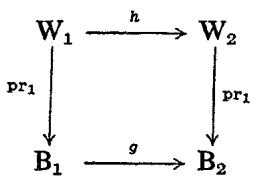
\includegraphics[keepaspectratio]{images/part001_9c3df15b.jpg}}

\(\mathbf{C}^{r}\) 类态射。设 \(\mathbf{W}_{1}\)（相应地，\(\mathbf{W}_{2}\)）是 \(\mathbf{B}_{1}\times\mathbf{F}_{1}\)（相应地，\(\mathbf{B}_{2}\times\mathbf{F}_{2}\)）的开子集，并设 \(h:\mathbf{W}_{1}\to\mathbf{W}_{2}\) 是一个映射。我们称 \(h\) 是一个 \(g\)-态射（\(\mathbf{C}^{r,s}\) 类的），如果 \(\mathrm{pr}_{1}\circ h=g\circ\mathrm{pr}_{1}\) 且 \(\mathrm{pr}_{2}\circ h\) 是 \(\mathbf{C}^{r,s}\) 类映射（15.1.6，从 \(\mathbf{W}_{1}\) 到 \(\mathbf{F}_{2}\)）。

类似地，设 \(B_{3}\) 是一个 \(C^{r}\) 类流形，\(W_{3}\) 是 \(B_{3} \times F_{3}\) 的开子集（其中 \(F_{3}\) 是一个 K-Banach 空间），并设 \(g'\) 是一个 \(C^{r}\) 类态射（从 \(B_{2}\) 到 \(B_{3}\)）。若 h（相应地，

\(h^{\prime})\)）是一个 \(g\)-态射（相应地，\(g^{\prime}\)-态射），是 \(\mathbf{C}^{r,s}\) 类的、从 \(\mathbf{W}_1\) 到 \(\mathbf{W}_2\)（相应地，从 \(\mathbf{W}_2\) 到 \(\mathbf{W}_3\)）的映射，则复合 \(h^{\prime} \circ h\) 是一个 \((g^{\prime} \circ g)\)-态射，是 \(\mathbf{C}^{r,s}\) 类的、从 \(\mathbf{W}_1\) 到 \(\mathbf{W}_3\) 的映射。

\subsection{\texorpdfstring{\(C^{r,s}\) 类流形（在 \(C^{r}\) 类流形之上）}{C\^{}\{r,s\} 类流形（在 C\^{}\{r\} 类流形之上）}}

在本节中，我们用 B 表示一个 \(C^{r}\) 类微分流形。

15.2.1. 设 X 是一个装备了映射 \(p: \mathbf{X} \to \mathbf{B}\) 的集合。我们称三元组 \(\theta = (\mathbf{V}, \psi, \mathbf{F})\) 为 X 在 B 上的卡，其中 V 是 X 的子集，F 是 K 上的 Banach 空间，\(\psi\) 是从 V 到 \(\mathbf{B} \times \mathbf{F}\) 的一个开子集上的双射，且满足 \(\mathrm{pr}_1 \circ \psi = p|\mathbf{V}\)。

设 \((\theta_{i})_{i\in I} = ((V_{i},\psi_{i},F_{i}))_{i\in I}\) 是 X 在 B 上的一个卡族。我们称诸 \(\theta_{i}\) 是 \(C^{r,s}\)-相容的，如果对 I 的每一对元素 \(i,j\)，下列两个条件都满足：

\begin{enumerate}
\def\labelenumi{\alph{enumi})}
\item
  \(\psi_i(V_i \cap V_j)\) 在 \(B \times F_i\) 中是开的，且 \(\psi_j(V_i \cap V_j)\) 在 \(B \times F_j\) 中是开的；
\item
  映射 \(\psi_i\circ\psi_j^{-1}\)（从 \(\psi_j(V_i\cap V_j)\) 到 \(\psi_i(V_i\cap V_j)\)）是一个 \(\mathrm{Id}_{\mathbf{B}}\)-态射，且是 \(\mathbf{C}^{r,s}\) 类的（15.1.7）。
\end{enumerate}

卡的一个族 \(((\mathrm{V}_i,\psi_i,\mathrm{F}_i))_{i\in I}\)（X 在 B 上的卡，它们 \(\mathbf{C}^{r,s}\)-相容且定义域 \(\mathrm{V}_i\) 覆盖 X）称为 X（在 B 上）的一个 \(\mathbf{C}^{r,s}\)-图册。两个 \(\mathbf{C}^{r,s}\)-图册称为等价的，如果它们的并仍是一个 \(\mathbf{C}^{r,s}\)-图册；\(\mathbf{C}^{r,s}\)-图册之间的等价关系是一个等价关系。\(\mathbf{C}^{r,s}\)-图册的一个等价类称为集合 X 上一个在 B 上的 \(\mathbf{C}^{r,s}\) 类流形结构；当希望指明 K 时，就写 \(\mathbf{C}_{\mathbb{K}}^{r,s}\) 以代替 \(\mathbf{C}^{r,s}\)。若 X 是 B 上的一个 \(\mathbf{C}^{r,s}\) 类流形，我们称 \(p\colon X\to B\) 为 X 的投影；若 \(\theta\) 是 X 在 B 上的一个卡，则我们称 \(\theta\) 是 \(\mathbf{C}^{r,s}\)-流形 X 的卡，如果 \(\theta\) 属于定义 X 结构的等价类中的某个图册。

设 X 是 B 上的一个 \(C^{r,s}\) 类流形，其投影为 p。则在 X 上存在

一个 \(\mathbf{C}^{r}\) 类微分流形结构，且是唯一的，使得对每个卡 \((V,\psi,F)\)（\(\mathbf{C}^{r,s}\)-流形 X 的卡），V 在 X 中是开的，且 \(\psi\) 是一个 \(\mathbf{C}^{r}\)-同构，它把 X 的开子流形 V 映到 \(\psi(V)\)（\(\mathbf{B}\times F\) 的开子流形）上。若给 X 装备这个结构，则映射 \(p:X\to B\) 是一个 \(\mathbf{C}^{r}\) 类的浸没。

设 \(b \in \mathbf{B}\)，并设 \(\mathbf{X}_b = p^{-1}(b)\)。存在一个 \(\mathbf{C}^s\) 类的 K-流形结构（\(\mathbf{X}_b\) 上的结构），且是唯一的，使得对每个卡 \(\theta = (\mathbf{V}, \psi, \mathbf{F})\)（\(\mathbf{C}^{r,s}\)-流形 \(\mathbf{X}\) 的卡），三元组 \(\theta_b = (\mathbf{V} \cap \mathbf{X}_b, \operatorname{pr}_2 \circ \psi | (\mathbf{V} \cap \mathbf{X}_b), \mathbf{F})\) 是流形 \(\mathbf{X}_b\) 的卡。这个结构之下的 \(\mathbf{C}^r\) 类微分流形结构是由上面定义的 \(\mathbf{C}^r\) 类微分流形结构（\(\mathbf{X}\) 上的结构）诱导的。
